\documentclass{article}

\usepackage{graphicx, amsmath}
\usepackage{subcaption}
\usepackage{float}
\usepackage{bm}

% 0. Referencing style, APA-like referencing
\usepackage[backend=biber, style=apa, natbib=true]{biblatex}
\usepackage{algorithm}
\usepackage{algorithmic}
\addbibresource{bibliography.bib}

% 1.  Don't need such wide margins.
\usepackage[margin=1in]{geometry} % Setting the margins to 1 inch

% \usepackage{amsmath}

\begin{document}

\title{Ordinal Data clustering and prediction}

\author{Quan Zhao}

\maketitle

% From VUW 487 Report
\section{Introduction}


The study of ordinal data presents unique challenges and opportunities.
Ordinal data consists of categories with an inherent order but undefined
spacing. This makes it distinct from nominal and continuous data,
necessitating specialized analytical methods that acknowledge its
structured ordering without presuming equal intervals between its
categories.

This project investigates methods for clustering and predicting cluster
membership for ordinal data. These methods are useful because ordinal
data is prevalent in fields ranging from social sciences to healthcare.
We begin by defining ordinal data and describing its distinctive
features. We then discuss existing clustering and prediction
methodologies. We focus on model-based clustering because we have an
existing sophisticated approach of this type, that is tailored to the
ordinal nature of the data, whereas there are limitations inherent in
distance-based methods when applied to ordinal data. The report
describes specific statistical models developed for ordinal data
analysis, such as the Proportional Odds model and the Ordered Stereotype
Model, highlighting their effectiveness in extracting meaningful
insights.

We then reflect on the historical development of ordinal data analysis,
from early methodologies to recent innovations that have broadened its
applicability and improved its precision. We also consider future
research directions, including the potential for integrating machine
learning with conventional statistical methods to refine the predictive
performance of ordinal data models.

Clustering methods have previously been developed for ordinal data,
using models such as the Ordered Stereotype Model. However, these
existing methods do not include techniques for determining the likely
cluster membership of any new observations that were not available at
the initial clustering stage. Therefore, this research aims to extend
these existing methods to accurately predict cluster membership for
incoming data points. Such advancements are crucial for applying ordinal
data in dynamic environments where new data are produced frequently. The
accuracy of the predictions is also important, so we will assess this to
ensure that the methods perform sufficiently well.

In summary, this paper offers an examination of methodologies for
clustering and predicting ordinal data. This inquiry is intended as a
resource for both researchers and practitioners, providing insights
necessary for navigating the complexities of ordinal data and leveraging
its full potential in analytical endeavors.

\subsection{Ordinal Data}

Ordinal data, a pivotal concept in statistical analysis, represents categorical data characterized by a meaningful order among its categories, without implying uniform differences between these ranks. Unlike nominal data, which merely categorizes without any implied ranking, ordinal data elevates the categorical analysis by introducing a hierarchy or sequence that is significant yet lacks quantifiable intervals between its elements. This characteristic distinguishes ordinal data: it conveys the sequence of values but remains silent on the magnitude of difference between successive ranks.

Such data often appear as rankings or ordered classifications where the precise distance between categories is undefined or irrelevant. 
Despite sometimes being numerically coded for analytical convenience, ordinal data resist traditional arithmetic operations, rendering calculations like addition or subtraction inappropriate and misleading.

In the realm of statistical analysis, ordinal data necessitates specialized, non-parametric methods. 
The median and mode stand out as appropriate measures of central tendency for this data types, 
aligning with their ordered nature without assuming equal intervals between categories.

Ordinal data's prevalence is notably high in social sciences, especially in surveys and questionnaires designed to capture subjective assessments such as attitudes, opinions, and preferences. These instruments frequently employ scales—ranging from ``strongly disagree'' to ``strongly agree''—to elicit responses that, while ordered, do not support the notion of fixed distances between adjacent categories. This principle underlines the core attribute of ordinal data: the clear hierarchy among responses without an inherent interval scale to quantify the gaps between them. Consequently, assigning numerical values to such categories for computational purposes is generally discouraged and conceptually flawed, as it misinterprets the data's ordinal nature 

(~\textcite{Johnson1999}) gives a good sample,
 It is typically rational to presume an order such as

 \[
 \text{strongly disagree} < \text{disagree} < \text{don’t know} < \text{agree} < \text{strongly agree}
\]
 However, it is often illogical to allocate integer values to these categories. Therefore, calculations like
\[
\text{``disagree''} - \text{``strongly disagree''}
\]

\[
\text{``agree''} - \text{``don't know''}
\]
are not considered valid. 
This demonstrates that performing arithmetic calculations on the numerical values assigned to the categories does not make sense.

% \begin{figure}[ht!] % 'h!' places the figure here, in the text
%     \centering % Centers the figure
%     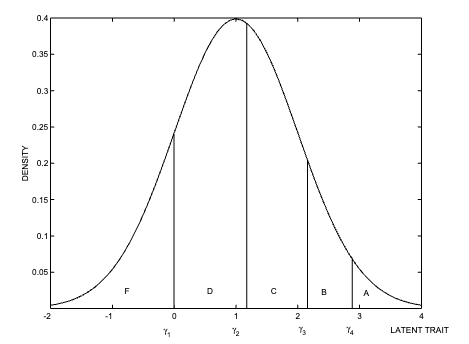
\includegraphics[width=0.6\textwidth]{images/ordinal_data_dist.png} % Include the image with 50% of the text width
%     \caption{Latent trait interpretation of ordinal classification. 
%     In this plot, the logistic density represents the distribution of latent traits for a particular individual. 
%     It is assumed that a random variable is drawn from this density, and the value of this random variable determines an individual's classification. 
%     For example, if a deviate of 0.5 is drawn, the individual receives a D. (~\cite{Johnson1999}).} % Caption for the image
%     \label{fig:ordinal} % Label for referencing the figure in the text
%   \end{figure}

\subsection{Comparison with continuous numerical data}

In the context of statistical analysis, the distinction between ordinal and continuous numerical data types is pivotal, influencing both the choice of analytical methods and the depth of insights that can be derived. 
Ordinal data, characterized by its capacity to rank order categories without indicating precise differences between them, is inherently less informative than continuous numerical data. 
Continuous numerical data, with its quantitative nature, allows for an infinite range of values and supports detailed statistical operations, including arithmetic calculations and the application of advanced statistical models, facilitating a nuanced understanding of variables and their interrelations (~\cite{Stevens1946}).

The limitations of ordinal data stem from its inability to quantify the exact magnitude of differences between categories, a factor that restricts the application of parametric statistical methods. This constraint necessitates reliance on non-parametric methods, focusing on medians and modes rather than means and standard deviations, thereby offering a less detailed analysis (~\cite{Conover1999}). 
For instance, in Likert scale responses commonly used in surveys, the ordinal nature of data precludes meaningful calculations of averages or differences between responses, limiting the depth of analysis that can be achieved (~\cite{Likert1932}).

Comparatively, continuous numerical data's capacity for precise measurement and the application of a broader range of statistical analyses enables a more detailed and accurate exploration of phenomena. 
This capability is contingent upon the availability of continuous numerical results, which may not always be feasible. The nature of the data collectible in certain research scenarios—such as measuring opinions, attitudes, or perceptions—often necessitates the use of ordinal data, due to the challenges associated with obtaining continuous measurements in these contexts. For instance, eliciting responses on a continuous percentage scale from 0 to 100 can be impractical when assessing subjective experiences or preferences. Hence, the decision to utilize ordinal data over continuous numerical data is not solely a matter of choice in research design and analysis but is also influenced by the practicalities of what data can realistically be gathered. This consideration is crucial for ensuring the validity and relevance of research findings, highlighting the importance of aligning data collection methods with the specific circumstances and constraints of the study.

In summary, while ordinal data is invaluable for capturing rankings and subjective assessments, 
its analytical limitations highlight the superior informational value of continuous numerical data in quantitative research. 
This distinction is crucial for researchers in the selection of appropriate statistical methods and in the interpretation of their data, 
ensuring that conclusions drawn are both valid and meaningful.

\subsection{Clustering}

Clustering is a fundamental technique in the field of data analysis and machine learning, aimed at grouping a set of objects in such a way that objects in the same group (or cluster) are more similar to each other than to those in other groups. Its applications span a wide range of areas including market research, pattern recognition, image analysis, and bioinformatics, among others. For instance, in market research, clustering can help identify distinct customer segments based on purchasing behavior, while in bioinformatics, it can be used to classify different types of genes or proteins with similar functions.

There are primarily two types of clustering: distance-based clustering and model-based clustering.

1. \textbf{Distance-based Clustering}: 

This approach relies on the concept of similarity or distance between data points. 
The aim is to minimize the distance between data points within a cluster while maximizing the distance between data points in different clusters. 
Popular methods include K-means (~\cite{macqueen1967some}), 
hierarchical clustering (~\cite{johnson1967hierarchical}), and DBSCAN (~\cite{ester1996density}), 
each using different metrics (e.g., Euclidean, Manhattan) to measure distance or similarity.

2. \textbf{Model-based Clustering}: 

Unlike distance-based methods, model-based clustering (~\cite{fraley2002model}) assumes that the data is generated from a mixture of finite distributions, 
where each component of the mixture represents a cluster. 
This approach tries to estimate the parameters of these distributions to optimize the fit between the model and the data. 
Model-based methods are particularly useful for complex data structures, including those with mixed types of data (numerical, categorical) or where the clusters have different sizes, shapes, or orientations.

Model-based clustering is often more suitable for ordinal data—data that contain natural, orderable categories. This is because ordinal data, which embody an inherent ranking or order (e.g., survey responses from "strongly agree" to "strongly disagree"), do not fit well with the distance metrics used in distance-based clustering, which treat distances between all pairs of categories as equal. Model-based clustering, on the other hand, can accommodate the ordinal nature by incorporating it into the model assumptions, allowing for a more nuanced understanding and grouping based on the inherent order of the data. This method can capture the ordinal information effectively, providing more meaningful and interpretable clusters for analysis.

\section{History of model-based Ordinal Data Clustering}

\subsection{Early Developments (2000--2010)}

McLachlan \& Basford 1988 (~\cite{mclachlan1988mixture}) start to marked a crucial step in mixture model applications by simplifying the maximum likelihood estimation (MLE) using the EM algorithm (~\cite{dempster1977maximum}).

McLachlan \& Peel's 2000 book further elaborate on this approach. This approach, utilizing $Y_j$ and $Z_j$, not only enhanced the computational efficiency of MLE but also laid a foundational strategy for Bayesian approaches and MCMC methods in mixture models. The paper’s impact is evident in its widespread adoption across various domains, from bioinformatics to finance, where mixture models are employed (~\cite{mclachlan2000finite}).

In 2002, Figueiredo's introduction of an unsupervised algorithm for learning finite mixture models was a game-changer. This method's ability to autonomously select the number of components represented a significant leap over previous techniques, which often relied on arbitrary or manual component selection. Additionally, the algorithm's robustness against initialization issues and singular estimates made it a go-to choice for practitioners dealing with complex multivariate data (~\cite{figueiredo2002unsupervised}).

A key paper in 2010 by Volodymyr and Ranjan addressed practical challenges in applying the EM algorithm for mixture models. This comprehensive guide to estimation, model selection, and likelihood maximization was a boon for both researchers and practitioners. Notably, the work extended beyond Gaussian mixtures, offering insights and methodologies for simulating and visualizing non-Gaussian mixtures, thereby broadening the applicability of mixture models (~\cite{10.1214/09-SS053}).

\subsection{Recent Developments (2010--2019)}

In 2016, Matechou et al. introduced a novel approach to data analysis with their proposal of finite mixture models for biclustering two-mode ordinal categorical data. Utilizing proportional odds parameterization, these models offered a sophisticated understanding of complex data patterns, particularly beneficial in fields such as genomics and social sciences where ordinal data is prevalent. The application of the EM algorithm for model fitting highlighted the continued importance of this method in the context of mixture model applications (~\cite{matechou2016biclustering}).

Similarly, in 2016, Fernandez et al. presented an alternative methodology for clustering ordinal data by employing likelihood-based methods through finite mixtures with the stereotype model. This approach stood out for its use in fuzzy clustering techniques, an area that has been attracting increased attention in the realm of data science (~\cite{fernandez2016mixture}).

In 2019 Fernandez et al.'s extension of finite mixture models to binary, count, and ordinal data under a unified statistical framework represented a consolidation and expansion of mixture model applications. The introduction of maximum likelihood estimation parameters and the Bayesian approach for simultaneous estimation were indicative of the field's progression towards more flexible and comprehensive modeling techniques (~\cite{fernandez2019finite}).

The primary innovation in both of these studies lies in the integration of ordinal data models with finite mixture methods, a departure from the traditional use of finite mixtures for continuous variables.


Jacques and Biernacki's 2018 introduction of a model-based co-clustering algorithm was a significant advancement. The algorithm's ability to handle missing data and its interpretability made it especially relevant for high-dimensional datasets. The BOS distribution employed in this model underscored the continuous innovation in probabilistic modeling techniques, catering to the increasing complexity of data in modern research (~\cite{jacques2018model}).

Compare with previous work, Jacques and Biernacki's (~\cite{jacques2018model}) method is based on a novel Binary Ordinal Search (BOS) model emphasizing efficiency and interpretability, especially with missing data. 

\subsection{Compare with other clustering algorithm}

Compared to tree based or distance based clustering algorithms, model-based clustering algorithms demonstrate superior performance with ordinal data, particularly in scenarios involving multiclass and multioutput cases. 
This advantage stems from two key factors: firstly, ordinal data do not presuppose equal distances between categories, a condition that distance-based methods often rely on. Secondly, ordinal data typically encompass only a few categories, which can limit the effectiveness of tree-based methods designed to partition data across a broader numerical range.

% End From VUW 487 Report

\section{Scope and Contributions of the latest project}

Building on the foundations laid by existing research on ordinal data, Finite Mixture Models (FMM), and the Ordered Stereotype Model (OSM), this paper aims to extend these methodologies to enable effective cluster prediction for unseen data. In particular, we develop an extension of the FMM framework to incorporate OSM, demonstrating how these methods can be applied not only to classify existing observations but also to predict cluster membership for new instances.

The primary contributions of this work are as follows:

\begin{enumerate}
    \item \textbf{Extension of FMM for Cluster Prediction}: We extend the FMM-based clustering model for ordinal data to provide predictive capabilities for new, unlabeled data. This is achieved by constructing a prediction function that, after estimating the model parameters from labeled training data, can directly assign cluster labels to new observations. The approach leverages the structure of the OSM to efficiently compute cluster probabilities, ensuring scalability and robustness in real-world applications.

    \item \textbf{Detailed Parameter Analysis}: We conduct a comprehensive examination of the components of the OSM, including the cluster effect, column effect, and covariate effect. This detailed analysis allows us to better understand how these parameters contribute to the clustering process, providing deeper insights into the interaction between different factors in the model.

    \item \textbf{Design and Validation through Simulation}: To empirically validate the effectiveness of the proposed method, we designed two types of data simulations: the OSM Simulation and the Normal Distribution Simulation. These simulations were used to test the model under various parameter settings, allowing us to evaluate the performance of the extended FMM across different scenarios. 

    \item \textbf{Replication Study for Stability}: To assess the stability and consistency of the proposed model, we conducted a replication study by running multiple experiments with different random seeds. This analysis provided insights into the robustness of the model under varying initial conditions, thereby demonstrating the reliability of our results.
\end{enumerate}

Overall, this paper presents a novel extension of the FMM framework that enables efficient cluster prediction for ordinal data, supported by rigorous experimentation and analysis. 
The findings contribute to the broader literature by expanding the application of FMM to predictive clustering tasks, offering new avenues for analyzing complex ordinal datasets.


\section{Statistical-based Ordinal Data Clustering}

\subsection{Ordered Stereotype Model}

The Ordered Stereotype Model, as introduced by Anderson (1984) (~\cite{anderson1984regression}), 
is a statistical approach specifically designed for analyzing ordinal dependent variables. 
These variables have categories that possess a natural order, 
though the differences between them are not directly quantifiable.

In this work, we adopt the methodology outlined by Fernández et al. (2016) (~\cite{fernandez2016mixture}). 
Let us consider an ordinal response variable \(Y_{ij}\) with categories denoted by \(k = 1, 2, \ldots, C\), 
where \(i\) represents the row index, and \(j\) represents the column index. 
The probability that \(Y_{ij}\) falls into the \(k\)-th category is given by \(P(Y = k)\). 
Suppose the data is partitioned into \(g\) clusters.

The model for the probability of category \(k\) is then expressed as follows:
\begin{equation}
  \log\left(\frac{P(Y = k| X)}{P(Y = 1| X)} \mid k \in C, g \in G, i \in n, j \in m\right) = \mu_k + \phi_k \times \left(\alpha_g + \beta_j + \bm{X}_i^T \cdot \bm{\delta} \right),
\end{equation}
where:

\begin{itemize}
    \item \(\mu_k\) is the intercept for category \(k\), with \(\mu_1\) set to zero to provide a reference category.
    \item \(\alpha_g\) represents the effect associated with cluster \(g\).
    \item \(\beta_j\) represents the effect associated with column \(j\).
    \item \(X\) is a d dimensional set of covariates.
    \item \(\delta\) represents the effect associated with covariates.
    \item \(X_i^T \cdot \delta\) represents the effect from the covariates associated with row \(i\), where \(\theta\) is a vector of coefficients.
\end{itemize}

A key feature of the Ordered Stereotype Model is the parameter \(\phi_k\), 
which must be arranged in an ordered sequence such that:
\[
0 = \phi_1 \leq \phi_2 \leq \ldots \leq \phi_q = 1.
\]
This constraint ensures that the model captures the natural ordering of categories, 
allowing the effects across different categories to follow a common, scaled pattern. 
The parameter \(\phi\) effectively adjusts the contribution of the predictors to the log-odds for each ordinal category, 
preserving the inherent structure of the ordinal response.

This modeling approach provides flexibility in representing the ordered nature of the data while maintaining interpretability, 
which is particularly useful for understanding the effects of cluster, row, and column factors in a unified framework.

  

% 123

\subsection{Expectation-Maximization (EM) Algorithm}

% EM algorithm has been introduced by Dempster, Laird and Rubin in 1977. (~\cite*[Dempster, Laird and Rubin]{Dempster1977}).

% The Expectation-Maximization (EM) algorithm is a two-step iterative method to obtain the maximum likelihood estimate (MLE) of the parameters of a statistical model, where the model depends on unobserved latent variables. The EM algorithm is particularly useful for mixture models, where the data is considered to be generated from a combination of several different statistical distributions, each representing a different 'component' of the population.

% \subsubsection*{Expectation-Maximization Algorithm for Mixture Model}

% A mixture model is a probabilistic model for representing the presence of subpopulations within an overall population, without requiring that an observed data set explicitly identify the subpopulation to which an individual observation belongs. Formally, if we assume a mixture of $K$ components, the probability density function (pdf) of a mixture model can be written as:

% \begin{equation}
% p(x|\Theta) = \sum_{k=1}^{K} \pi_k f_k(x|\theta_k)
% \end{equation}

% where $x$ represents the data points, $\Theta$ represents the parameters of the mixture model which include both the mixing coefficients $\pi_k$ and the parameters of the component distributions $\theta_k$, $f_k$ is the component distribution, and $\pi_k$ are the mixing coefficients such that $\sum_{k=1}^{K} \pi_k = 1$ and $\pi_k \ge 0$.

% \subsubsection{Introduction to the EM Algorithm}
The Expectation-Maximization (EM) algorithm is a powerful statistical tool for finding maximum likelihood estimates in models with latent variables. It consists of two main steps: the Expectation step (E-step) and the Maximization step (M-step).

In the context of clustering within a finite mixture model, the EM algorithm considers cluster assignments as latent variables. 
The EM algorithm for mixture models assumes that a set of latent variables $Z$ indicate which component of the mixture each observation originates from.

During the E-step, the algorithm estimates the expected value of the log-likelihood function, with respect to the conditional distribution of the latent variables given the observed data and the current estimates of the parameters. This step can be formally expressed as follows:
\begin{equation}
Q(\theta | \theta^{(t)}) = E_{Z|X, Y, \theta^{(t)}}[\log L(\theta; X, Y, Z)]
\end{equation}
where \( \theta \) denotes the parameter vector, \(X \) respresents the covariates, \( Y \) represents the observed data, \( Z \) are the latent variables, \( L \) is the likelihood function, and \( \theta^{(t)} \) are the parameter estimates from the previous iteration.

In the M-step, the algorithm maximizes the expected log-likelihood found in the E-step with respect to the parameters to obtain new parameter estimates:
\begin{equation}
\hat{\theta}^{(t+1)} = \arg \max_{\theta} Q(\theta | \theta^{(t)})
\end{equation}

\subsubsection{E-step (Expectation Step)}

During the Expectation step, the EM algorithm computes the expected value of the log likelihood function, with respect to the conditional distribution of the latent variables given the observed data under the current estimate of the parameters. This step involves calculating the posterior probabilities that a given data point belongs to each of the $G$ components, based on the current estimates of the parameters.

For a mixture model, the posterior probability (also known as the responsibility) that observation i originates in component g is calculated as:

\begin{equation}
\hat{Z}_{ig} = \frac{\pi_g f_g(\mathbf{y_i}|\theta_g)}{\sum_{j=1}^{G} \pi_j f_j(\mathbf{y_i} \mid \theta_j)}
\end{equation}

\subsubsection{M-step (Maximization Step)}

In the Maximization step, the EM algorithm updates the parameters of the model to maximize the expected log likelihood using the latest latent values $Z_{ig}$ from the E step. 
This involves updating the estimates of both the parameters of the component distributions and the mixing coefficients.

Update the mixing coefficients:

\begin{equation}
\hat{\pi}_g^{new} = \frac{1}{N} \sum_{i=1}^{N} \hat{Z}_{ig}
\end{equation}

The remaining parameters are updated using numerical optimization.

% 2. Update the parameters of the component distributions ($\theta_k$), which depends on the form of the distribution. For example, in a Gaussian mixture model, the mean and covariance of each Gaussian component are updated as follows:

% \begin{equation}
% \mu_k^{new} = \frac{\sum_{i=1}^{N} \gamma(z_{ik}) x_i}{\sum_{i=1}^{N} \gamma(z_{ik})}
% \end{equation}

% \begin{equation}
% \Sigma_k^{new} = \frac{\sum_{i=1}^{N} \gamma(z_{ik}) (x_i - \mu_k^{new})(x_i - \mu_k^{new})^T}{\sum_{i=1}^{N} \gamma(z_{ik})}
% \end{equation}

% where $N$ is the total number of data points.

% abc

% \section{Expectation-Maximization Algorithm for Clustering in Finite Mixture Models}


\section{Cluster Prediction for Ordinal Data}

Finite mixture models, combined with ordered stereotype regression, offer a technique for cluster prediction in ordinal data analysis. This method posits that a population can be probabilistically segmented into more homogeneous clusters, potentially enhancing prediction accuracy.

In our study, we will concentrate on row clusters with (Ordered Stereotype Model) OSM as an example to demonstrate our prediction method. It is feasible to apply this approach to other types, such as column clusters, or to models like POM.

\subsection{Data Structuring and Model Training}

The observed data ($Y$) is divided into a training set ($Y'$) and a test set ($Y''$). The training set comprises the first $t$ observations for adjusting model parameters, while the subsequent observations ($y_{t+1}, \dots, y_n$) make up the test set for evaluating the model.

The Expectation-Maximization (EM) algorithm is used to refine the parameters of the finite mixture model using the training data. 
Here, $k$ represents the number of ordinal categories, and $g$ denotes the number of clusters. 
The aggregate probability for each category, summed across all clusters, must equal one.

During the training phase, the M-step of the EM algorithm updates the parameters, 
$\mu_k$ and $\phi_k$ for each category, $\alpha_g$, $\beta_j$ and $\theta$ for each cluster.

Upon completion of the EM algorithm, we obtain their estimates $\hat{\mu}_k$, $\hat{\phi}_k$, $\hat{\alpha}_g$, $\hat{\beta}_j$ and $\hat{\theta}$ which are utilized for cluster prediction.

To achieve our objectives, the implementation will utilize the "clustord" package (\cite{clustord2024}), 
developed by the School of Mathematics and Statistics at Victoria University of Wellington. 
This package integrates the Ordered Stereotype Model (OSM) (\cite{fernandez2016mixture}), the Proportional Odds Model (POM) (\cite{matechou2016biclustering}), and several binary methods (\cite{pledger2014multivariate}), 
providing the ability to fit clustering models incorporating a wide array of covariates.

In our research, the parameter training stage for the OSM, as facilitated by the clustord package, is conducted following Fernandez's methodology (\cite{fernandez2016mixture}).

\subsection{Prediction and Validation}

After training, in the prediction stage the prediction will be applied in each row of the new data.

The posterior probability of row $i$ being in cluster g is:

% \begin{equation}
% PP_irg = \sum_{L}^{j=1} e^{\mu_k + \phi_k \cdot \alpha_g}
% \end{equation}

\begin{equation}
  \hat{Z}_{ig} = \frac{\hat{\pi}_g f_g(\mathbf{y_i}|\hat{\theta}_g)}{\sum_{j=1}^{G} \hat{\pi}_j f_j(\mathbf{y_i} \mid \hat{\theta}_j)}
\end{equation}

Then, the prediction of the cluster of row would be maximum $\hat{Z}_{ig}$ over all clusters g.

The model's accuracy is measured by how well the predicted clusters match the actual test data classifications.

\section{Data Simulations to understanding the parameters}

In this section, we conduct experiments based on data generated from specified OSM parameters to analyze the effects of cluster and category distributions.

% \subsection{OSM (Ordered Stereotype Model) Simulation}
We systematically vary individual model parameters while holding others constant to observe their influence on data density, particularly focusing on the parameter $\alpha$. The default parameters used in the simulations are as follows:
\[
\begin{aligned}
G &= 2, \\
q &= 3, \\
\alpha &= \mathbf{c}(1, -1), \\
\beta &= \mathbf{c}(0), \\
\mu &= \mathbf{c}(0, 0, 0), \\
\phi &= \mathbf{c}(0, 0.5, 1), \\
\pi &= \mathbf{c}(0.5, 0.5).
\end{aligned}
\]
All parameters except for $\beta$ are applied to a single outcome variable $Y$. This approach allows us to demonstrate the effects of adjusting a specific parameter on data density.

\subsection{Effect of Different $\alpha$ Values}
In the OSM framework, $alpha$ is the argument of clusters. the sum of the $\alpha$ parameters is constrained to equal zero. 
We examine the impact of varying the $\alpha$ values using the following configurations:
\[
\begin{aligned}
\alpha_1 &= \mathbf{c}(-0.1, 0.1), \\
\alpha_2 &= \mathbf{c}(-1, 1), \\
\alpha_3 &= \mathbf{c}(-3, 3).
\end{aligned}
\]
We set cluster 1 has negitive $alpha$ value and cluster 2 has postive value.
As shown in Figure~\ref{fig:alpha}, 
the cluster has high $alpha$ value leading to have larger probability to have sample in high category.
And cluster has lower $alpha$ value have larger probability to have sample in low category.

\begin{figure}[htbp!]
  \centering
  \begin{subfigure}{1.0\textwidth}
      \centering
      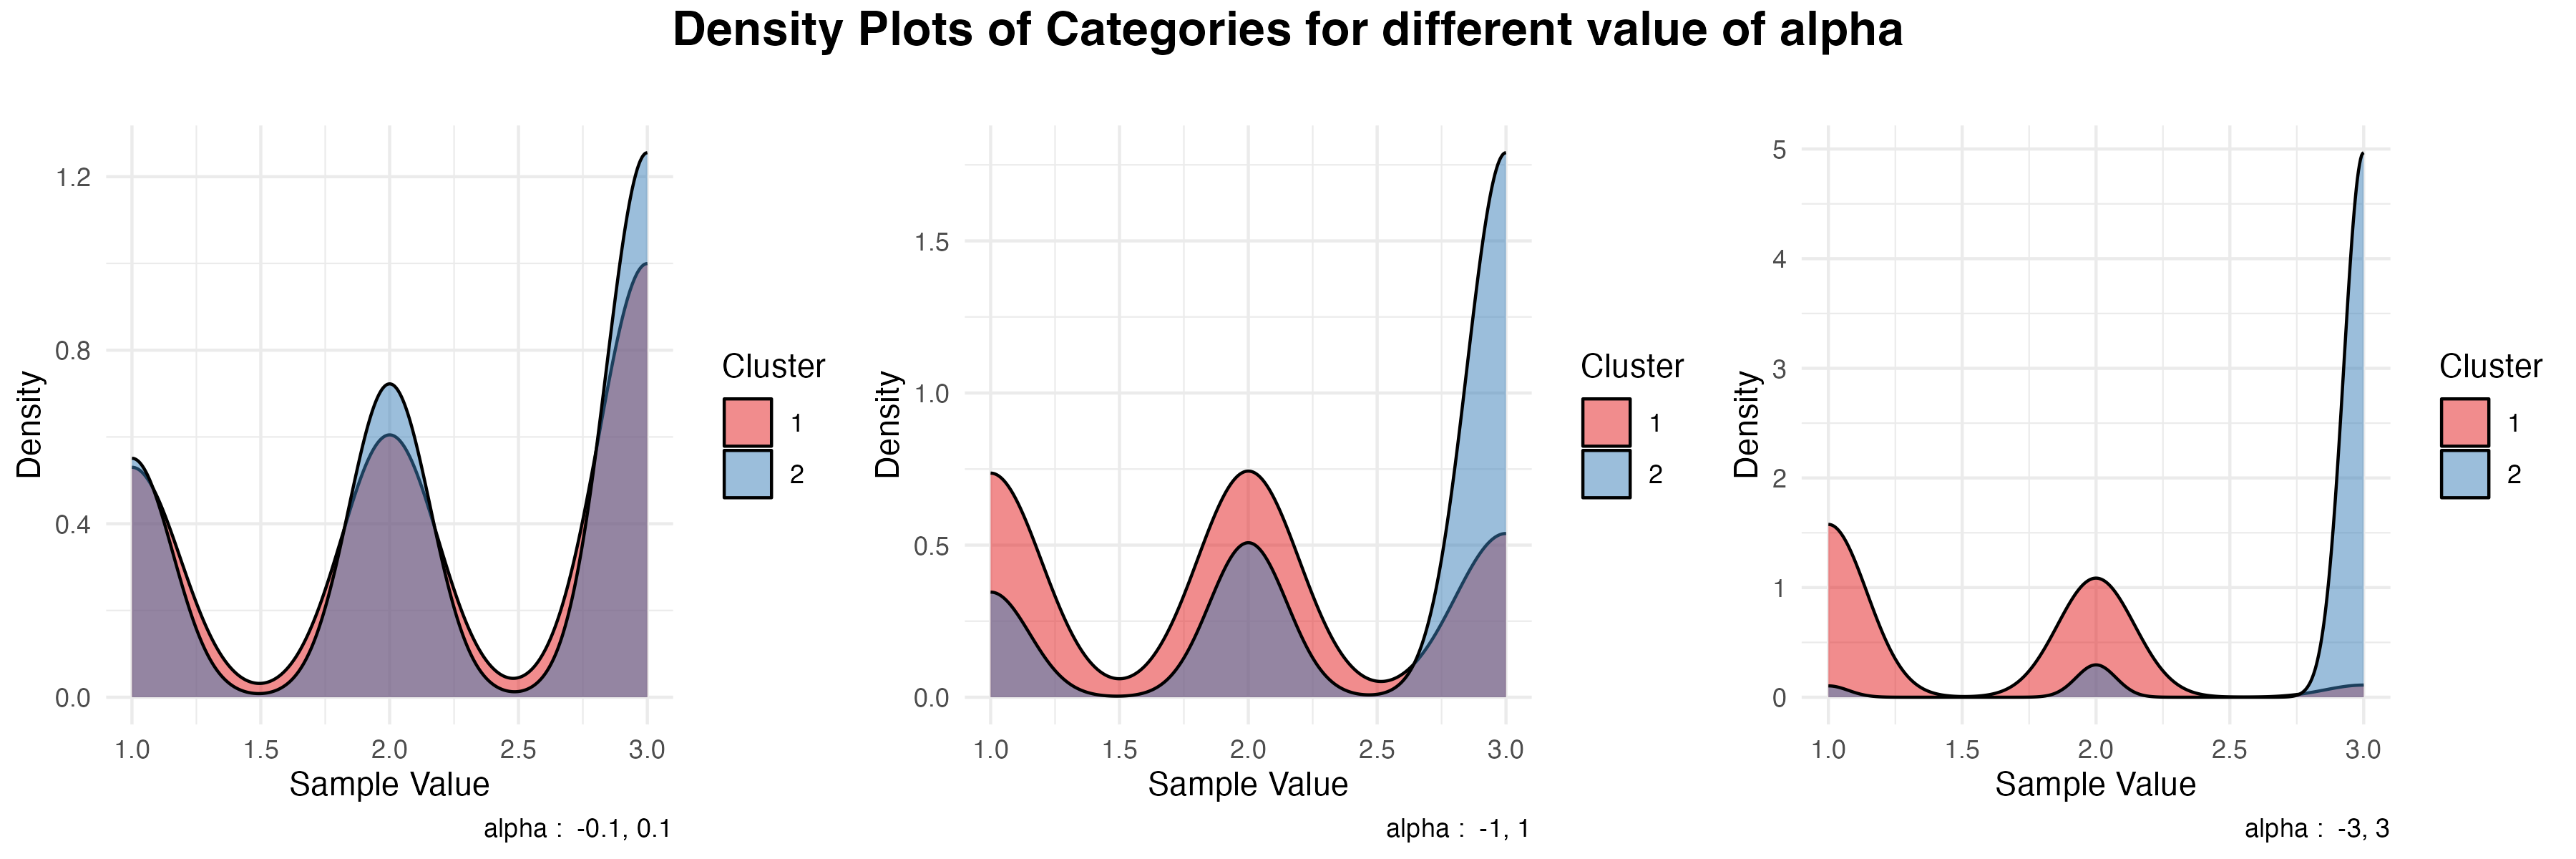
\includegraphics[width=\textwidth]{images/para_sim/alpha.png}
  \end{subfigure}
  \caption{effect to cluster distribution from difference $\alpha$ value}
  \label{fig:alpha}
\end{figure}

% mu
\subsection{Effect of Different $\mu$ Values}
In OSM, $mu$ is argument of category. 
The first value must be zero. There is no value limitation of $mu$, it can be large or negative.
To investigate the impact of varying $\mu$ values on the cluster distributions, 
we consider the following configurations:
\[
\begin{aligned}
\mu_1 &= \mathbf{c}(0, -1, -2), \\
\mu_2 &= \mathbf{c}(0, 2, 1), \\
\mu_3 &= \mathbf{c}(0, 1, 2).
\end{aligned}
\]
Figure~\ref{fig:mu} illustrates the effects of different $\mu$ value.
It shows the category has high $mu$ value leading to high probability of sample.
we also can see, $\mu_1$ and $\mu_3$ plots are showing left and right mirror. 
and the $\mu_2$ is in the middle.
( TODO: This is related to defalut $phi$ value. 
Need to check the detial reason.)

\begin{figure}[htbp!]
  \centering
  \begin{subfigure}{1.0\textwidth}
      \centering
      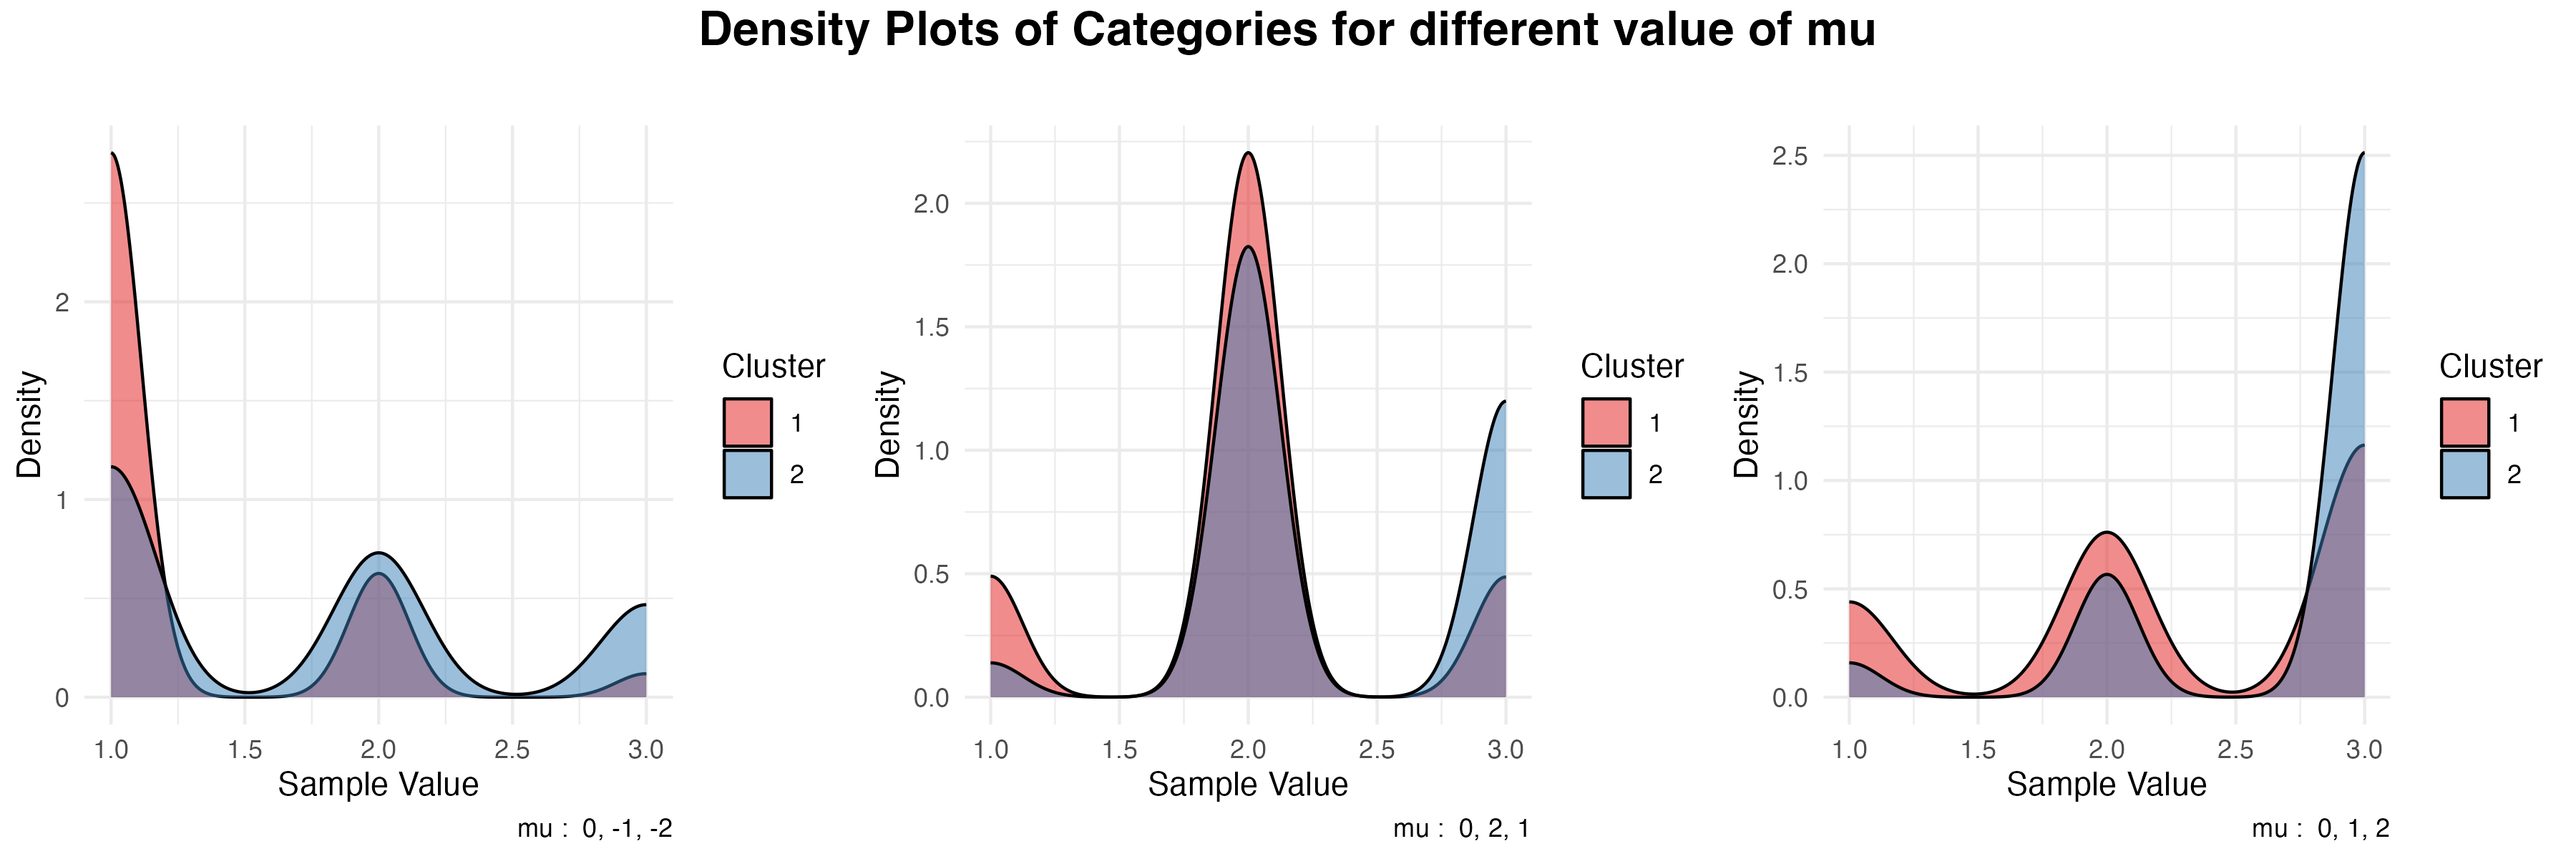
\includegraphics[width=\textwidth]{images/para_sim/mu.png}
  \end{subfigure}
  \caption{effect to cluster distribution from difference $\mu$ value}
  \label{fig:mu}
\end{figure}

\clearpage

% phi
\subsection{Effect of Different $\phi$ Values}
The parameter $\phi$ represents the ordinal effect for each category, reflecting the cumulative probability across ordered categories. 
Importantly, the $\phi$ values must start from 0 and the $\phi$ value of the last category must be 1. 
To evaluate the impact of different $\phi$ values, we consider the following configurations:
\[
\phi_1 = \mathbf{c}(0, 0.2, 1), \quad \phi_2 = \mathbf{c}(0, 0.5, 1), \quad \phi_3 = \mathbf{c}(0, 0.8, 1).
\]
As shown in Figure~\ref{fig:phi}, 
when the probability associated with the second category increases (as $\phi$ values rise), 
the density distribution changes significantly between the clusters. 
Specifically, in Cluster 1, there is a slight decrease in the density of the second category, 
while Cluster 2 exhibits a clear increase in the density of the same category. 
This indicates that higher $\phi$ values lead to a greater disparity 
in the density distributions between the clusters, 
particularly affecting the category with the increased $\phi$ value.

Overall, these results suggest that larger $\phi$ values amplify the differences in density between categories across clusters, 
with a more pronounced effect on the cluster associated with the higher $\phi$ values.

\begin{figure}[htbp!]
  \centering
  \begin{subfigure}{1.0\textwidth}
      \centering
      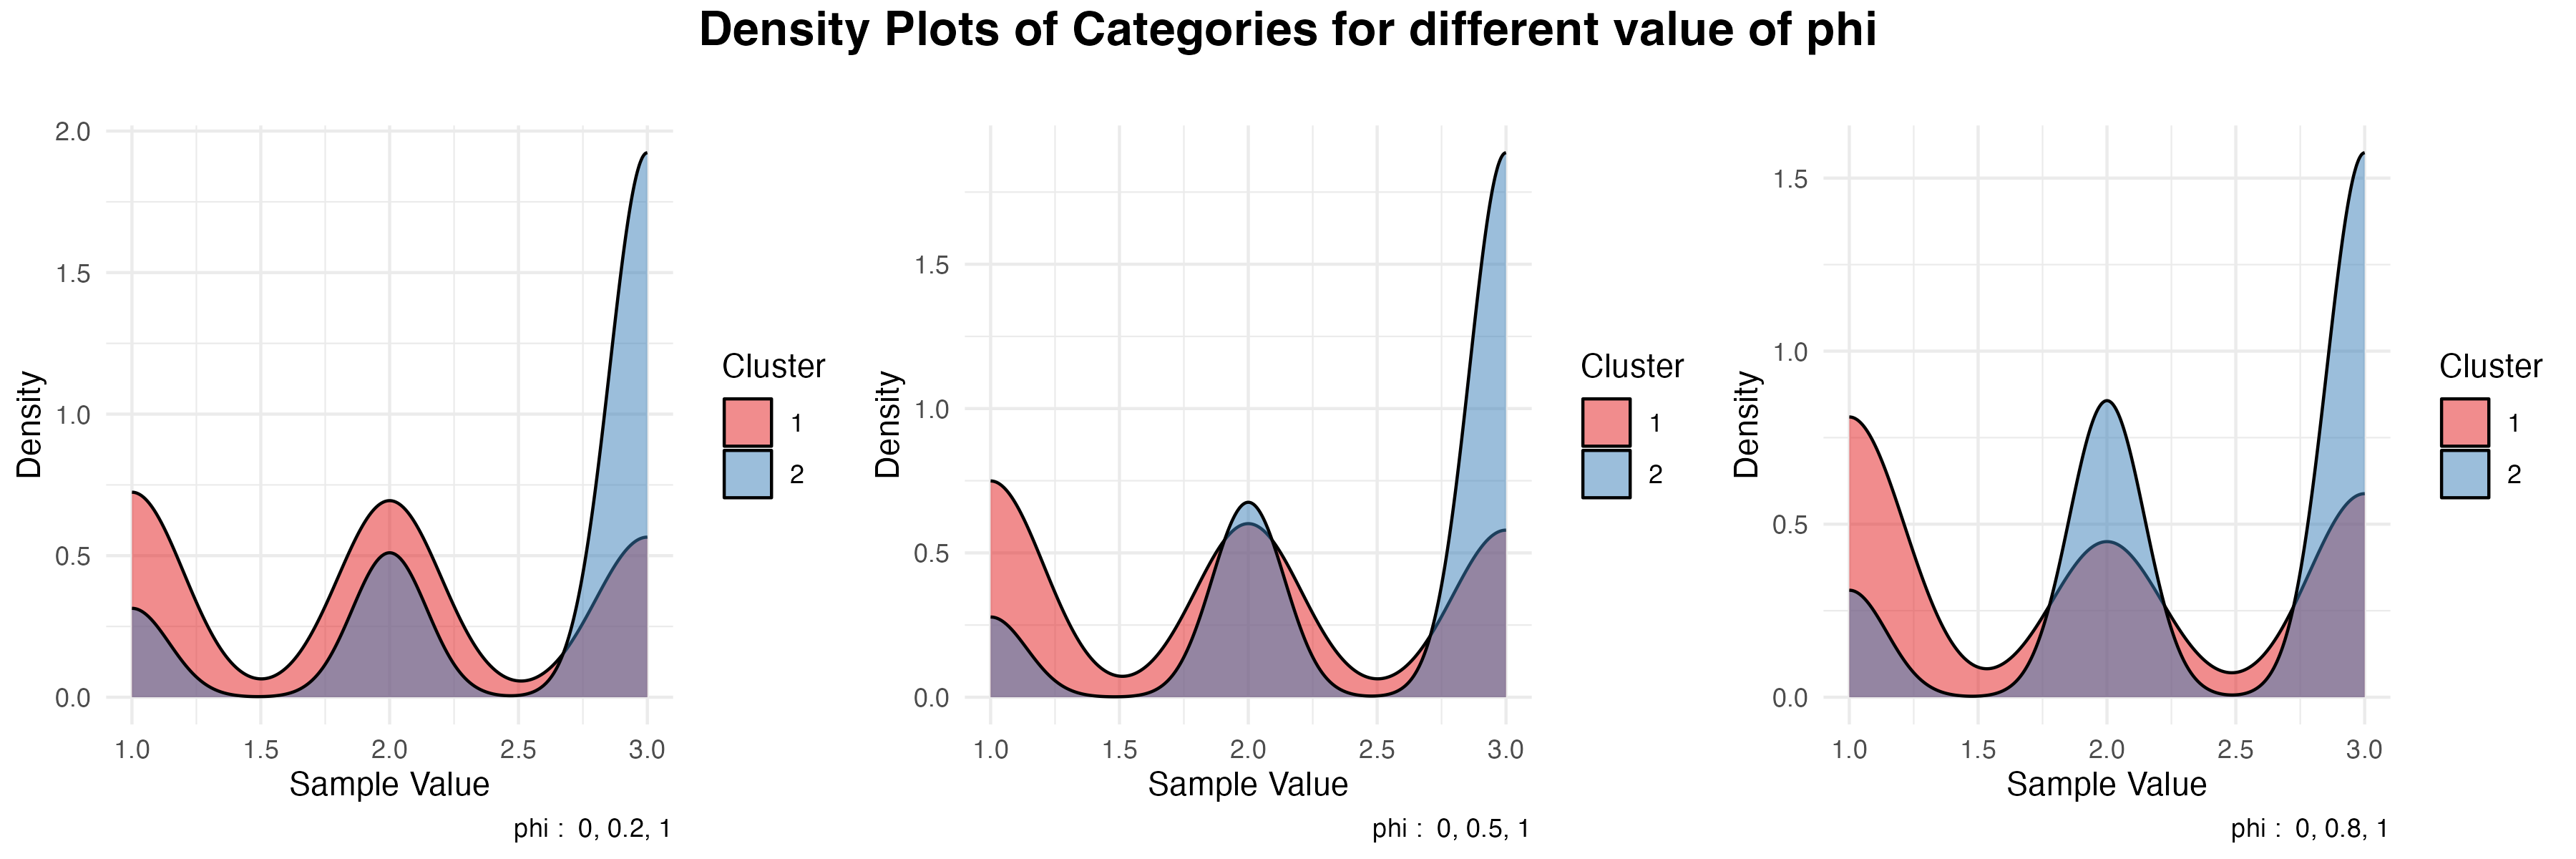
\includegraphics[width=\textwidth]{images/para_sim/phi.png}
  \end{subfigure}
  \caption{effect to cluster distribution from difference $\phi$ value}
  \label{fig:phi}
\end{figure}

% beta
\subsection{different $\beta$ value}
The parameter $\beta$ represents the effect of each column in the data. 
Figure~\ref{fig:beta} illustrates three different sets of $\beta$ values across five columns. 
When the $\beta$ values are close to zero, the impact on the data distribution is minimal. 
In Figure~\ref{fig:beta} a, the sampling distributions are nearly identical to the scenario where $\beta = 0$, 
indicating no significant effect from the columns. 
As we compare Figures~\ref{fig:beta} a, b, and c, it becomes evident that the effects 
from the columns increase as the $\beta$ values deviate further from zero.

Additionally, negative $\beta$ values result in a higher probability of sampling from the lower categories, 
whereas positive $\beta$ values increase the likelihood of sampling from the higher categories.
\begin{figure}[htbp!]
  \centering
  \begin{subfigure}{1.0\textwidth}
      \centering
      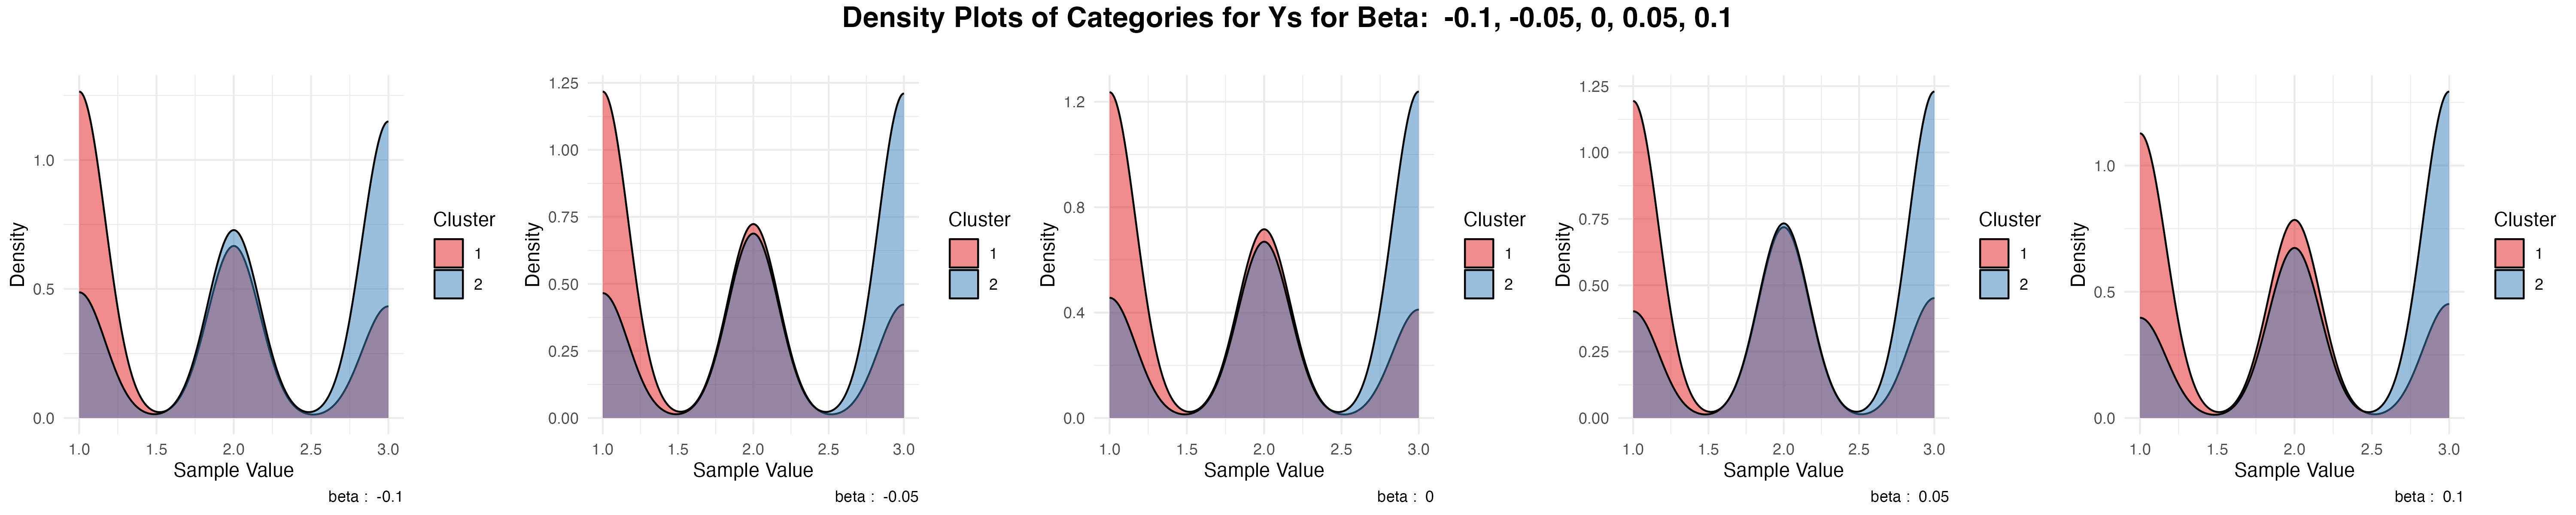
\includegraphics[width=\textwidth]{images/para_sim/beta_1.png}
      \caption*{a. samll difference between $\beta$}
  \end{subfigure}

  \begin{subfigure}{1.0\textwidth}
      \centering
      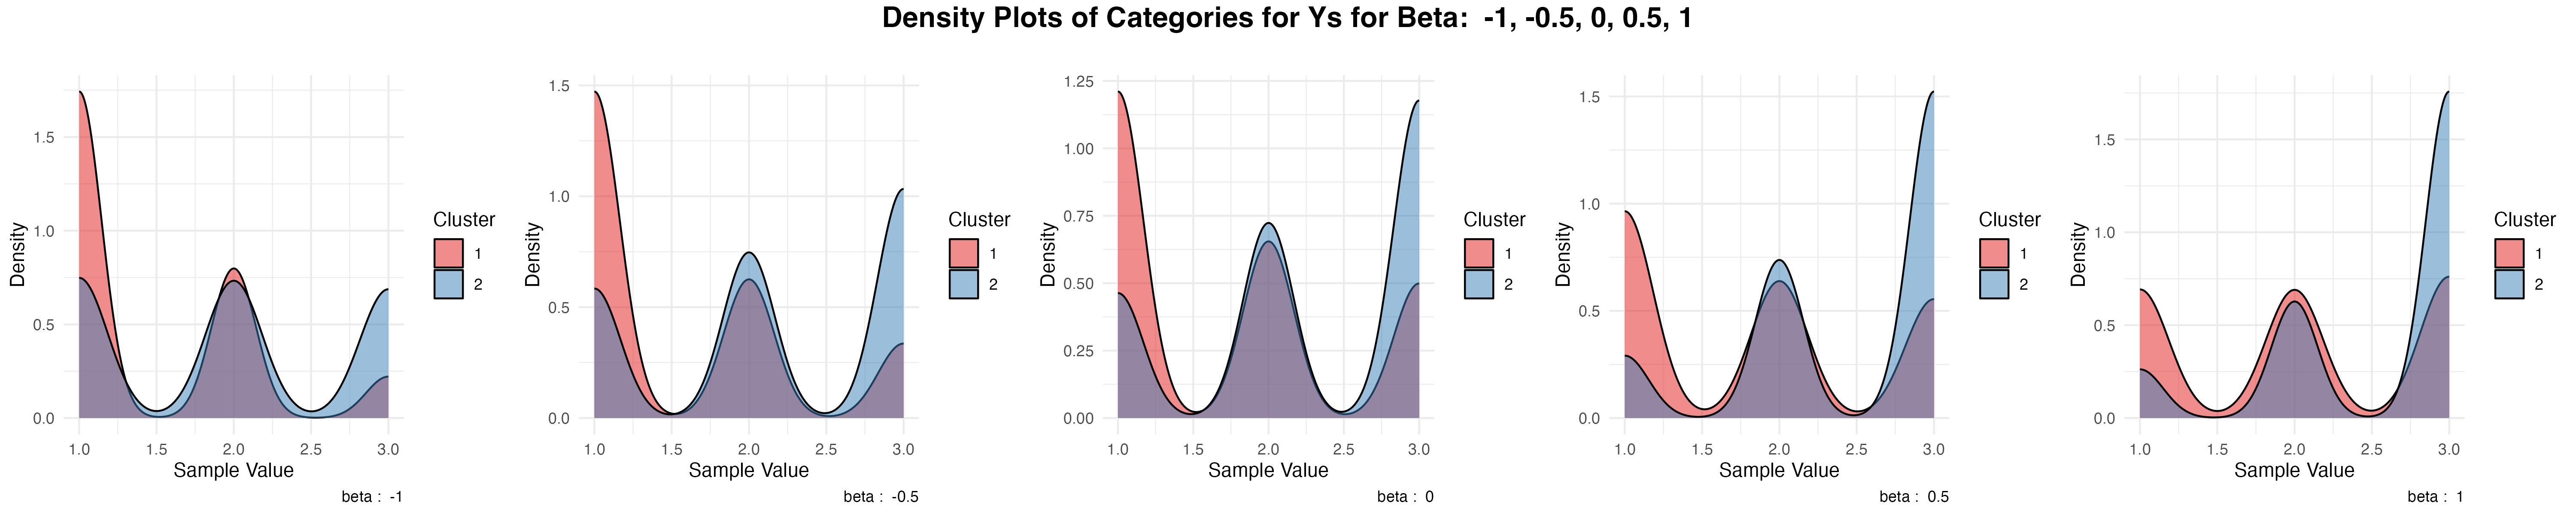
\includegraphics[width=\textwidth]{images/para_sim/beta_2.png}
      \caption*{a. medim difference between $\beta$}
    \end{subfigure}

  \begin{subfigure}{1.0\textwidth}
      \centering
      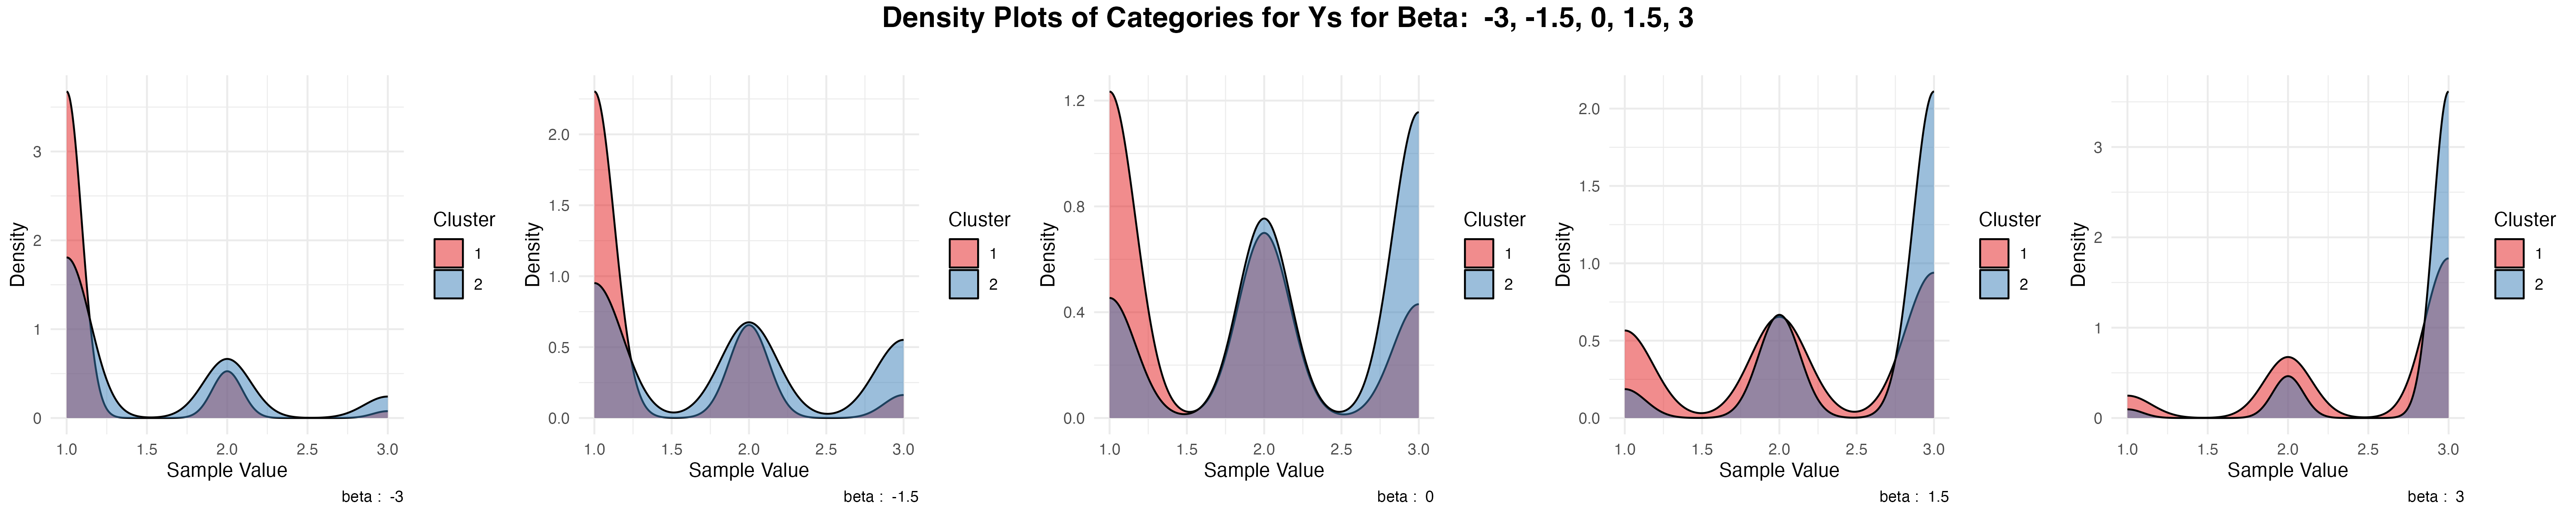
\includegraphics[width=\textwidth]{images/para_sim/beta_3.png}
      \caption*{a. large difference between $\beta$}
  \end{subfigure}
  
  \caption{Effect to cluster distribution from different $\beta$ values}
  \label{fig:beta}
\end{figure}

\clearpage

% pi
\subsection{Effect of Different $\pi$ Values}
In EM Algorithm, the $\pi$ parameter effects the sample size of each cluster. 
In Figure~\ref{fig:pi} shows when $\pi$ value small leading to less sample size.
when $\pi$ larger then the cluster has more sample size.
When $\pi$ same then the overall sample size is close.
\begin{figure}[htbp!]
  \centering
  \begin{subfigure}{1.0\textwidth}
      \centering
      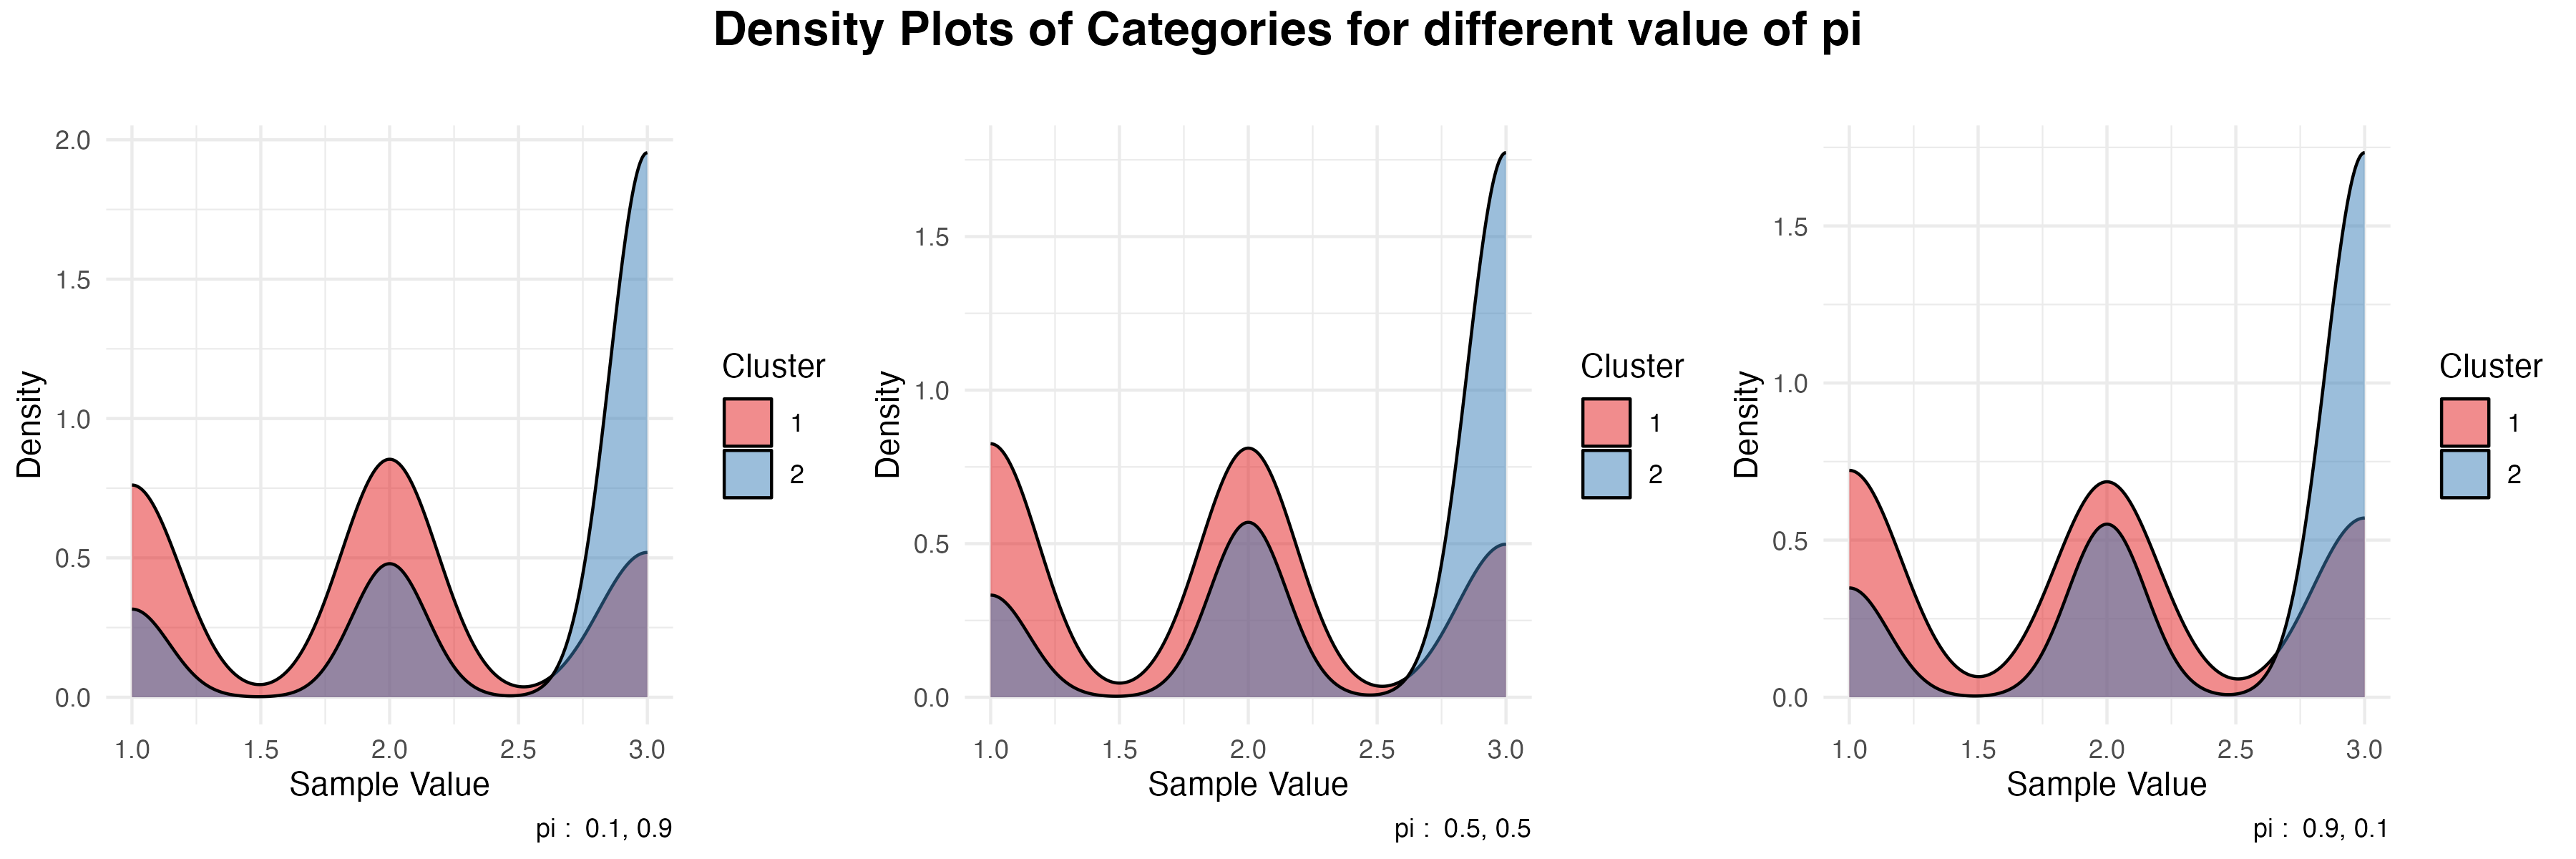
\includegraphics[width=\textwidth]{images/para_sim/pi.png}
  \end{subfigure}
  \caption{effect to cluster distribution from difference $\pi$ value}
  \label{fig:pi}
\end{figure}

% Normal Dist Simu Section
\section{Ordinal Data Simulations by Normal Distributions}

In order to better simulate the actual situation.
In this work, we introduced another approach to simulation the ordinal data 
for our prediction experiments. 
This approach is based on assume the data in each cluster are following 
a known distribution with known parameter of that distribution.
And the value of each categories are selected by cuts which same to each clusters.

In Cluster distributions, our work is based on two clusters and three categories.

There are 3 difference cluster distributions settings, which shown in 

Figure~\ref*{fig:dist_sim} (a) clusters follow different distribution with closer means $N(0,6)$ and $N(3,8)$
with same two cuts at $0$ and $2.5$,

Figure~\ref*{fig:dist_sim} (b) clusters follow different distribution with medium means $N(-1,1)$ and $N(-1.5,2)$
with same two cuts at $-1$ and $1$,

Figure~\ref*{fig:dist_sim} (c) clusters follow different distribution with far means $N(0,1)$ and $N(4,2)$
with same two cuts at $1$ and $2.5$,

\begin{figure}[htbp!]
  \centering
  \begin{subfigure}{0.32\textwidth}  % Adjust width to 0.32 to fit three images in a row
    \centering
    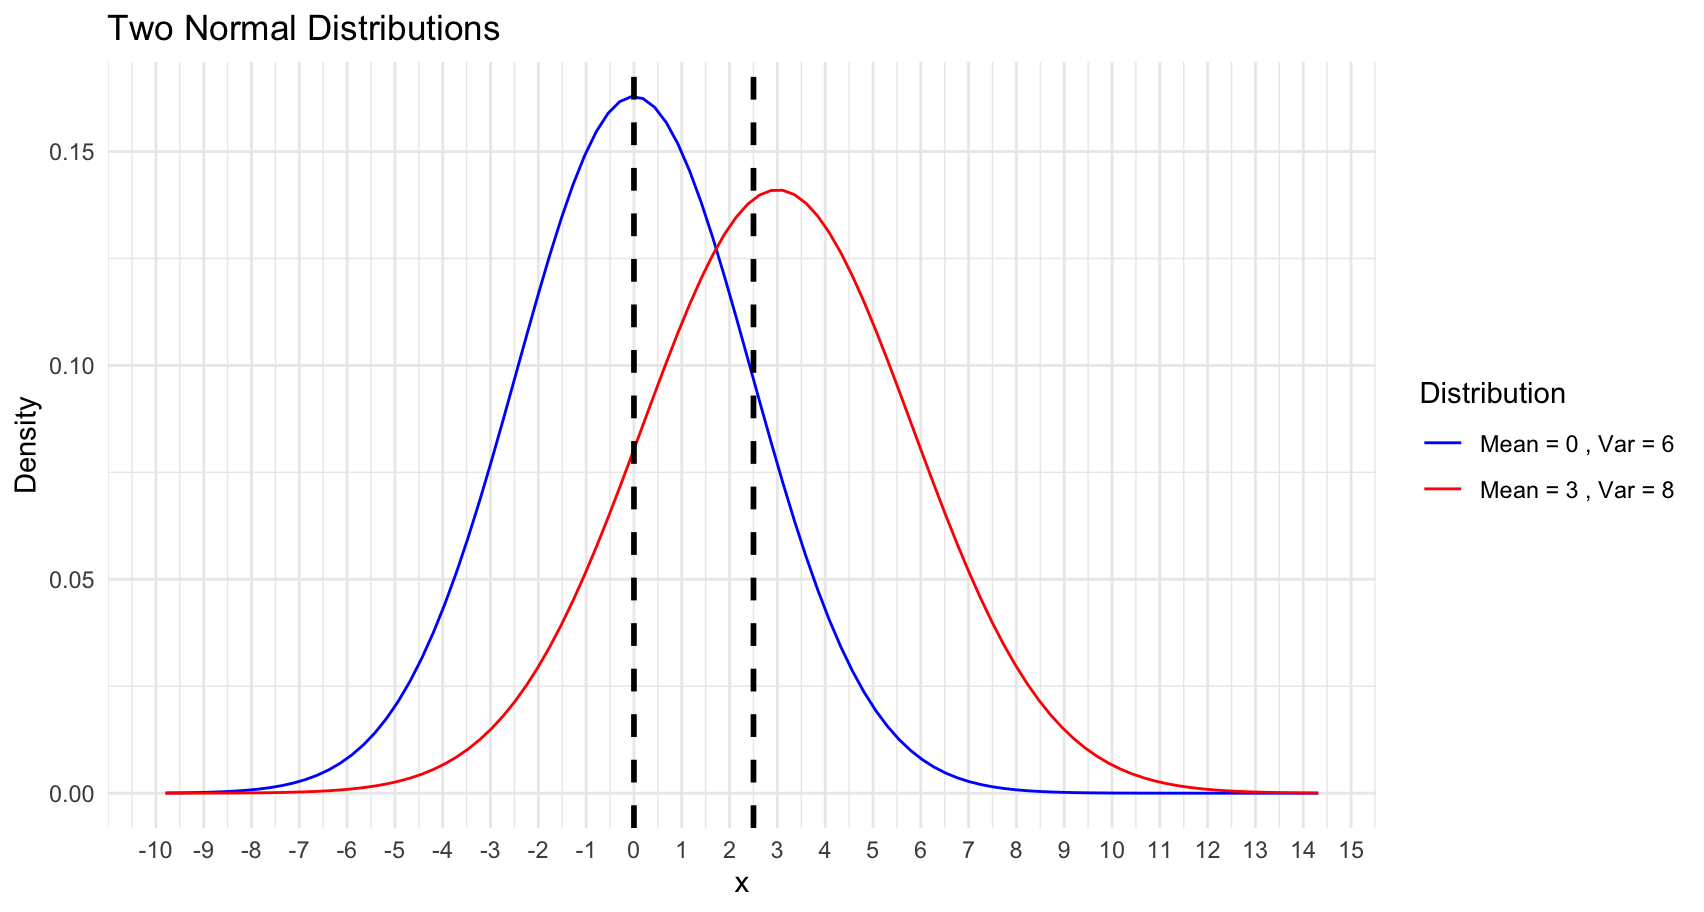
\includegraphics[width=\textwidth]{images/dist_simu/nor_close.png} % Replace with your second image path
    \caption{Clusters follow different distribution with close centre\\ cut1=0, cut2=2.5}
\end{subfigure}
  \hfill
  \begin{subfigure}{0.32\textwidth}  % Adjust width to 0.32 to fit three images in a row
    \centering
    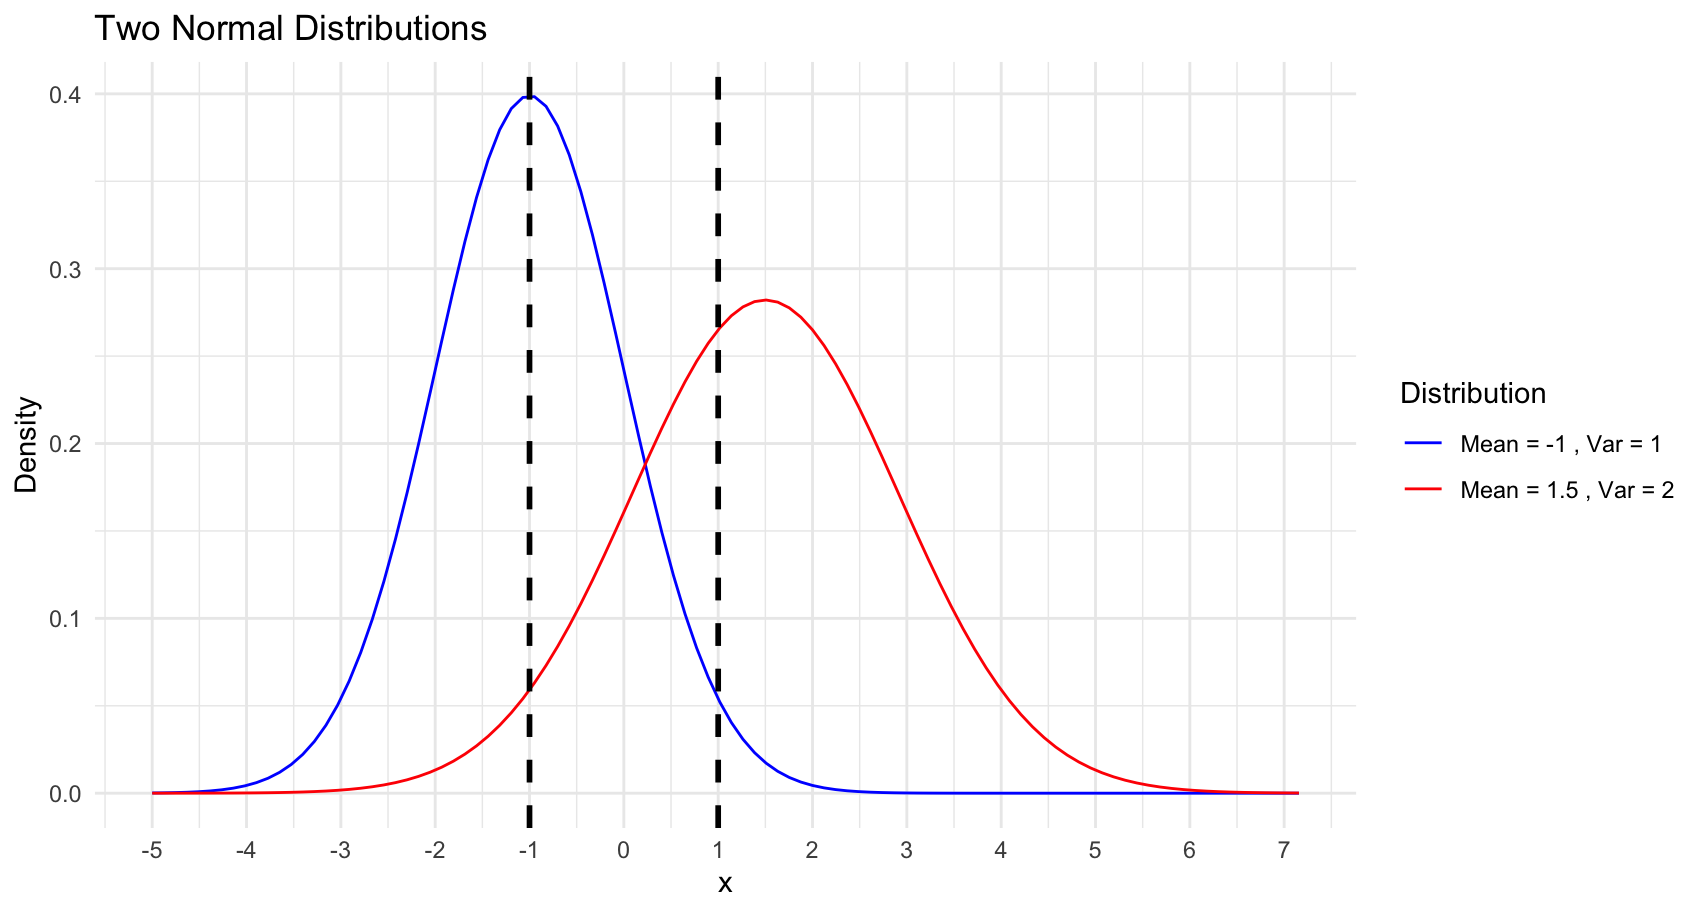
\includegraphics[width=\textwidth]{images/dist_simu/nor.png} % Replace with your first image path
    \caption{Clusters follow different distribution with medium distance centre\\ cut1=-1, cut2=1}
\end{subfigure}
  \hfill
  \begin{subfigure}{0.32\textwidth}  % Adjust width to 0.32 to fit three images in a row
      \centering
      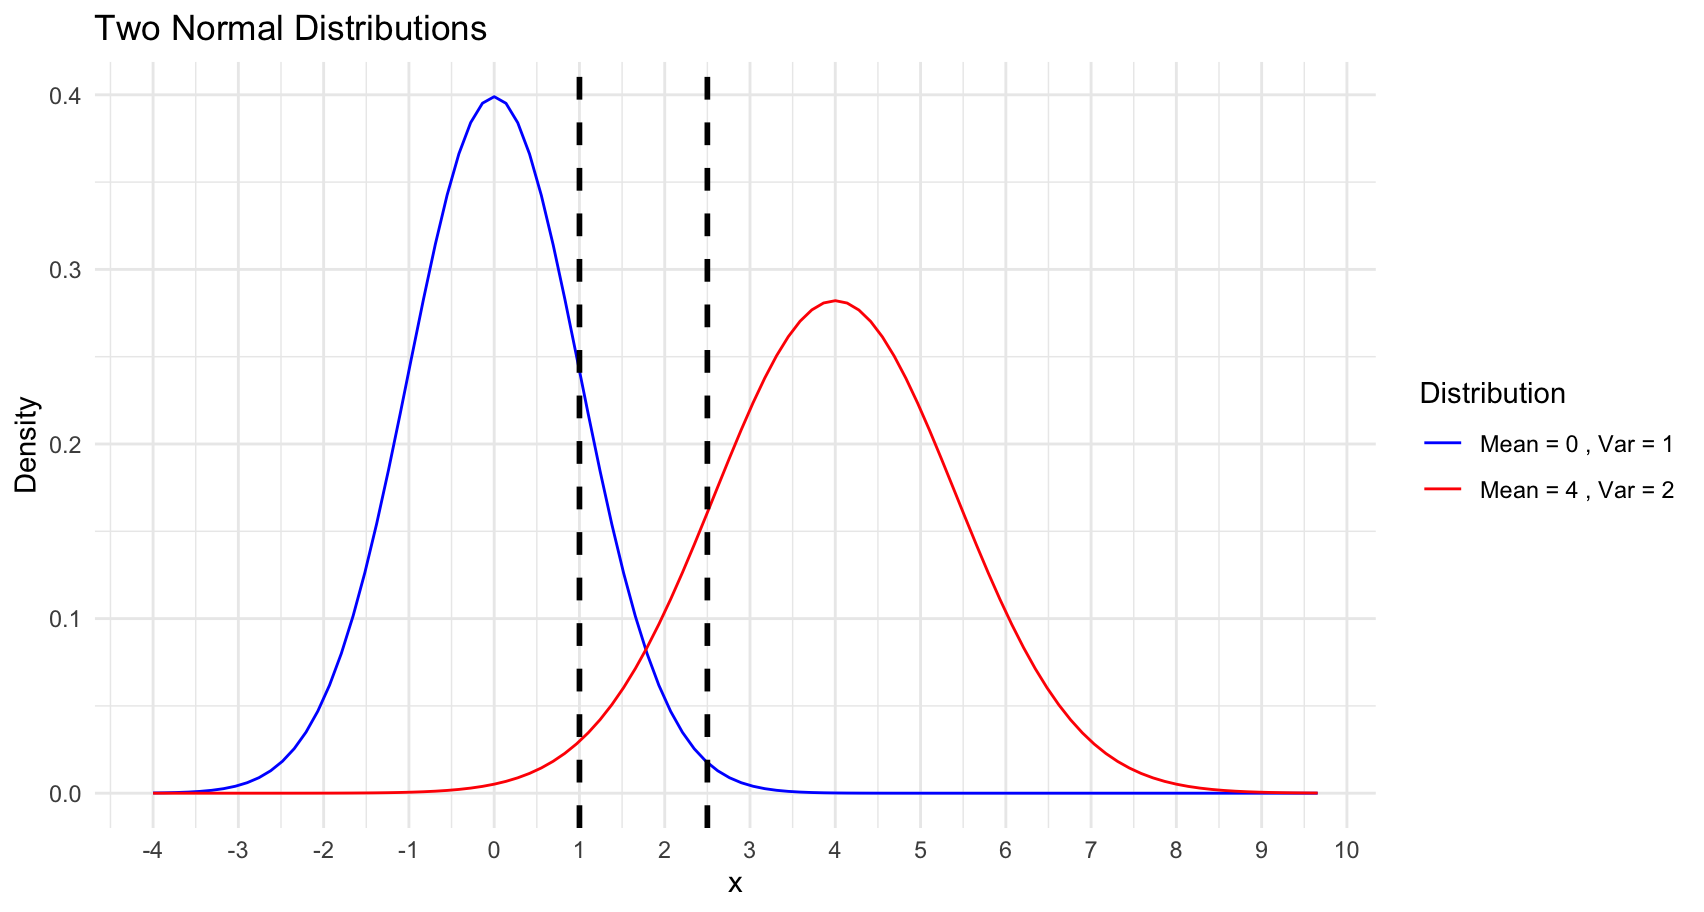
\includegraphics[width=\textwidth]{images/dist_simu/nor_far.png} % Replace with your third image path
      \caption{Clusters follow different distribution with far centre\\ cut1=1, cut2=2.5}
  \end{subfigure}
  
  \caption{Normal Distribution Simulations: with 3 clusters. the sample value if less then cut 1 is category 1, between cut 1 and cut 2 is category 2, and larger than cut 2 is category 3.}
  \label{fig:dist_sim}
\end{figure}


\section{Experiments approach}

In this study, we divided the simulated data into training and validation sets.

First, We use clustord R packagae \cite{clustord2024} to fit the parameters by the Expectation-Maximization (EM) algorithm was applied to estimate the parameter values from the training data, using only the response variable $Y$.

Next, the procedure outlined in Algorithm~\ref{fig:algo} was employed to calculate the probability of each category, cluster, column and row combination for each new observation in the validation set.

Finally, for each new observation $Y'$ in the validation set, we computed the Z-score for each cluster using these standardized probabilities.

Additionally, the defalut parameter given by EM algorithm have label switching problem.
The label switching is the cluster parameter $\alpha$ not in a correct order, which leading the prediciton logic given wrong prediction.
% TODO add reference and given more formal definition of "label switching"
In this work we reordering the fitted clusters in order of decreasing $\alpha$ then do predictions based on the reordered clusters.

\begin{algorithm}
  \caption{Pseudocode for Calculating Cluster Probabilities}
  \label{fig:algo}
  \begin{algorithmic}[1]
  \STATE Initialize a 4D array \texttt{cluster\_probs} with dimensions $G \times \texttt{number\_of\_row} \times \texttt{number\_of\_y} \times q$ and all elements set to 0.
  
  \FOR{$g = 1$ to $G$}
      \FOR{$i = 1$ to \texttt{number\_of\_row}}
          \FOR{$j = 1$ to \texttt{number\_of\_y}}
              \FOR{$k = 1$ to $q$}
                  \IF{$k > 1$}
                      \STATE Calculate $\texttt{linear} \gets \mu[k] + \phi[k] \times (\alpha[g] + \beta[j] + \sum \delta \times X[i,])$
                      \STATE Set $\texttt{cluster\_probs}[g, i, j, k] \gets \exp(\texttt{linear})$
                  \ELSE
                      \STATE Set $\texttt{cluster\_probs}[g, i, j, k] \gets 1$
                  \ENDIF
              \ENDFOR
              \STATE Normalize $\texttt{cluster\_probs}[g, i, j, :]$ by dividing each element by the sum of all elements in that row.
          \ENDFOR
      \ENDFOR
  \ENDFOR
  
  \RETURN \texttt{cluster\_probs}
  \end{algorithmic}
\end{algorithm}

\subsection{Handling Label Switching in Model Predictions}

One of the common issues encountered in clustering analysis, 
particularly when using probabilistic models such as the Expectation-Maximization (EM) algorithm, 
is the phenomenon known as "label switching." 

Label switching occurs when the clustering algorithm assigns different cluster identifiers (labels) to similar data points across different runs, 
even though the underlying clustering structure remains consistent. 
This can be particularly problematic in evaluating the consistency of ordinal data predictions, 
as correct predictions may receive mismatched cluster labels, 
thereby obscuring the true performance of the model.

In this work, we address the issue of label switching by implementing a post-processing step to reorder the estimates of cluster-specific parameters, 
specifically the estimated probability of the latent variable 
$\alpha$, produced by the EM algorithm. By reordering these probability estimates, 
we ensure that the cluster labels are aligned consistently across multiple runs, 
thereby maintaining interpretability and allowing for a more accurate assessment of model performance.

The reordering process is performed based on the values of the estimated probabilities of 
$\alpha$, ensuring that clusters are always labeled in a consistent manner—e.g., 
from the smallest to the largest probability value. 
This deterministic relabeling method effectively mitigates the label switching problem, 
allowing us to accurately evaluate the correspondence between predicted clusters and the true structure of the data.

Through this approach, we are able to compare cluster assignments across different experiments without ambiguity, 
ensuring that the predicted labels are not arbitrarily permuted, and thereby enhancing the reliability of our model evaluation. 
This is particularly critical for ordinal data, where maintaining the natural ordering of the clusters is essential for meaningful interpretation.


\section{Experiment Results}

These experiments were designed to assess the suitability of the Ordered Stereotype Model (OSM) for predicting clusters within ordinal data, specifically exploring its potential application within a Finite Factor Mixture Model (FFM) framework. In the OSM simulations, we examined the model’s predictive capability across a range of parameter configurations, including variations in the number of response variables and clusters. This setup allowed us to systematically observe how the model's accuracy responds to changes in data volume and clustering complexity, providing insights into its robustness in distinguishing clusters within ordinal datasets.

Conversely, the Normal Distribution simulations aimed to evaluate the model’s performance under conditions that more closely mirror real-world scenarios, where data often follows a particular distribution. By simulating data with Normal distributions, we analyzed the model’s effectiveness in classifying observations based on typical distributional structures, offering a complementary perspective on its clustering performance in structured data environments.

Finally, we compared the outcomes of the OSM and Normal Distribution simulations to assess the model’s consistency and adaptability across different simulation types. This comparison offers a comprehensive understanding of the model’s strengths and limitations in handling diverse data distributions and clustering complexities, thereby clarifying its practical utility for clustering ordinal data in FFM applications.
\subsection{Prediction with OSM simulate}

\subsubsection*{Prediction with Different Numbers of \( Y \) Values}

This experiment aims to evaluate the effect of different numbers of response variables (\( Y \)) on the clustering performance of the Ordered Stereotype Model (OSM). The parameters used in this experiment are as follows:

\[
\begin{aligned}
G &= 2, \\
q &= 3, \\
\alpha &= \mathbf{c}(1, -1), \\
\mu &= \mathbf{c}(0, 0, 0), \\
\phi &= \mathbf{c}(0, 0.5, 1), \\
\pi &= \mathbf{c}(0.5, 0.5).
\end{aligned}
\]

Additionally, the covariate effect, \(\beta\), was generated from a uniform distribution over the interval \([-1, 1]\):

\[
\beta \sim \mathcal{U}(-1, 1)
\]

For the 20 \( Y \) experiment, we generated 20 values of \(\beta\), while for the 30 and 50 \( Y \) experiments, 30 and 50 values of \(\beta\) were generated, respectively. 
The confusion matrices for these experiments are shown in Tables~\ref{tab:20_ys}, \ref{tab:30_ys}, and \ref{tab:50_ys}, demonstrating the model's clustering prediction results for different numbers of response variables.

From Figure~\ref{fig:exp_res}(a), we observe a clear trend: as the number of \( Y \) values increases, the prediction accuracy also improves. 
This improvement suggests that a larger number of response variables provides more information for distinguishing between clusters, leading to better model performance. 
Specifically, the prediction accuracy increased from 0.96 for 20 \( Y \) values to 0.9983 for 50 \( Y \) values, indicating that the availability of more covariate data enhances the clustering capability of the model.

TODO: ADD 20, 30, 50 Ys for 5 clusters

\subsubsection*{Prediction with Different Numbers of Clusters}

In the second set of experiments, we investigated the impact of varying the number of clusters while keeping other parameters constant. 
The experiments were conducted with 2, 3, and 5 clusters, and the default parameter values were used across all cluster configurations, with 20 values of \( Y \) generated for each experiment. 
The EM algorithm was configured with the following parameters: EM cycles = 100, start EM cycles = 5, and nstarts = 5.

For the three-cluster experiment, the values of \(\alpha\) were set to \(-1, 0, 1\), and the cluster proportions (\(\pi\)) were set to 0.33, 0.34, and 0.33, respectively. 
In the five-cluster experiment, \(\alpha\) values were set to \(-1, -0.5, 0, 0.5, 1\), with equal cluster proportions of 0.2 for each cluster. 
The confusion matrices for the different cluster configurations are presented in Tables~\ref{tab:2_clu}, \ref{tab:3_clu}, and \ref{tab:5_clu}.

Figure~\ref{fig:exp_res}(b) illustrates the overall prediction accuracy for different numbers of clusters. 
It is evident that as the number of clusters increases, the prediction accuracy decreases significantly. 
The model achieved an accuracy of 0.96 for 2 clusters, while the accuracy dropped to 0.2461 for 5 clusters. 
This rapid decline in accuracy can be attributed to the increased complexity introduced by a larger number of clusters, which requires more information to accurately distinguish between them. 
With only 20 \( Y \) values, the information available was insufficient to clearly differentiate among 5 clusters, leading to decreased performance.

\subsubsection*{Summary and Observations}

Overall, the experiments demonstrate that the number of response variables (\( Y \)) and the number of clusters (\( G \)) have a significant impact on the clustering performance of the Ordered Stereotype Model. 
Increasing the number of \( Y \) values provides more information to the model, resulting in improved clustering accuracy. 
However, as the number of clusters increases, the complexity of the clustering task also increases, and the model requires a larger amount of information to maintain high accuracy.

The results highlight the importance of appropriately selecting the number of response variables and clusters to ensure the model performs effectively. 
When the number of clusters is high, more response variables are necessary to capture the complexity of the data and achieve reliable cluster predictions. 
This finding is crucial for practical applications where the model's performance depends on balancing the granularity of clustering with the availability of data.

\begin{figure}[htbp!]
  \centering
  \begin{subfigure}{0.49\textwidth}
      \centering
      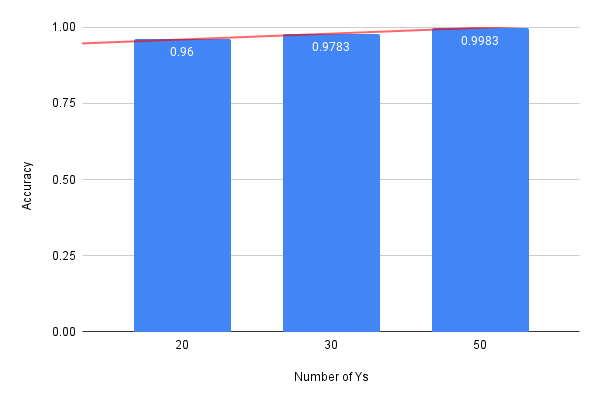
\includegraphics[width=\textwidth]{images/experiments/dif_ys.png}
      \caption{Prediction Accuracy of 2 clusters with different number of Ys}
  \end{subfigure}
  \hfill
  \begin{subfigure}{0.49\textwidth}
      \centering
      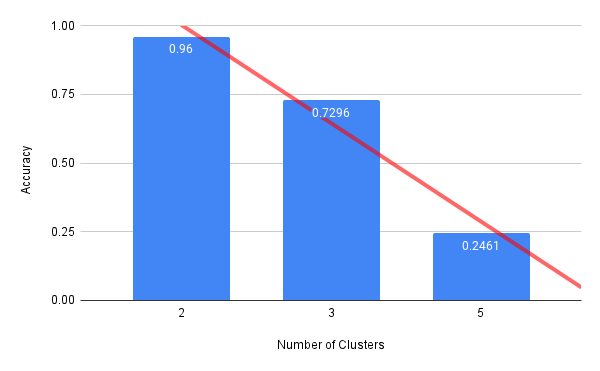
\includegraphics[width=\textwidth]{images/experiments/exp_diff_clusters.png} % Replace with your second image path
      \caption{Prediction Accuracy of different number of Clusters with 20 Ys}
  \end{subfigure}
  \caption{Cluster Prediction Experiments Results}
  \label{fig:exp_res}
\end{figure}

\begin{table}[htbp!]
  \centering

  % Title above all tables
  \caption*{\textbf{Confusion matrix of 2 clusters different number of Ys}}

  % First row of tables (2 side by side)
  \begin{minipage}{0.45\textwidth}
    \centering
    \begin{tabular}{c|c|c|c}
              & \textbf{Reference} & 1 & 2 \\
    \hline
    \textbf{Prediction} & 1 & 283 & 0 \\
                        & 2 & 15 & 293 \\
    \end{tabular}
    \caption{20 Ys}
    \label{tab:20_ys}
  \end{minipage}
  \hfill
  \begin{minipage}{0.45\textwidth}
    \centering
    \begin{tabular}{c|c|c|c}
              & \textbf{Reference} & 1 & 2 \\
    \hline
    \textbf{Prediction} & 1 & 289 & 4 \\
                        & 2 & 9 & 298 \\
    \end{tabular}
    \caption{30 Ys}
    \label{tab:30_ys}
  \end{minipage}
  
  \vspace{1em} % Space between rows
  
  % Second row (1 table centered)
  \begin{minipage}{0.6\textwidth}
    \centering
    \begin{tabular}{c|c|c|c}
              & \textbf{Reference} & 1 & 2 \\
    \hline
    \textbf{Prediction} & 1 & 297 & 10 \\
                        & 2 & 1 & 302 \\
    \end{tabular}
    \caption{50 Ys}
    \label{tab:50_ys}
  \end{minipage}

\end{table}

% confustion matrix of diff clusters

\begin{table}[htbp!]
  \centering

  % Title above all tables
  \caption*{\textbf{Confusion matrix of different number of Clusters with 20 Ys}}

  % First row of tables (2 side by side)
  \begin{minipage}{0.45\textwidth}
    \centering
    \begin{tabular}{c|c|c|c}
              & \textbf{Reference} & 1 & 2 \\
    \hline
    \textbf{Prediction} & 1 & 283 & 0 \\
                        & 2 & 15 & 293 \\
    \end{tabular}
    \caption{2 Clusters}
    \label{tab:2_clu}
  \end{minipage}
  \hfill
  \begin{minipage}{0.45\textwidth}
    \centering
    \begin{tabular}{c|c|c|c|c}
      & \textbf{Reference} & \textbf{1} & \textbf{2} & \textbf{3} \\
      \hline
      \textbf{Prediction} & \textbf{1} & 334 & 63 & 0 \\
                          & \textbf{2} & 110 & 383 & 152 \\
                          & \textbf{3} & 1 & 39 & 268 \\
    \end{tabular}
    \caption{3 Clusters}
    \label{tab:3_clu}
  \end{minipage}
  
  \vspace{1em} % Space between rows
  
  % Second row (1 table centered)
  \begin{minipage}{0.6\textwidth}
    \centering
    \begin{tabular}{c|c|c|c|c|c|c}
      & \textbf{Reference} & \textbf{1} & \textbf{2} & \textbf{3} & \textbf{4} & \textbf{5} \\
      \hline
      \textbf{Prediction} & \textbf{1} & 0 & 0 & 0 & 0 & 0 \\
                          & \textbf{2} & 505 & 201 & 69 & 6 & 0 \\
                          & \textbf{3} & 0 & 0 & 0 & 0 & 0 \\
                          & \textbf{4} & 243 & 543 & 730 & 722 & 731 \\
                          & \textbf{5} & 0 & 0 & 0 & 0 & 0 \\
    \end{tabular}
    \caption{5 Clusters}
    \label{tab:5_clu}
  \end{minipage}

\end{table}

\clearpage

\subsubsection{Analysis of 8-Cluster Prediction Performance}

The prediction accuracy for the 8-cluster experiment was notably low, as shown in the confusion matrix and the overall accuracy statistic (see Table~\ref{tab:8_clu}). This result can be attributed to the mismatch between the number of clusters and the amount of information available from the response variable \(Y\).

In this experiment, we attempted to identify 8 distinct clusters using only 20 values of \(Y\). This setup presented a significant limitation: the small number of \(Y\) values did not provide sufficient information to effectively distinguish between a large number of clusters. As a result, the model struggled to accurately differentiate all 8 clusters, leading to poor prediction performance.

The confusion matrix in Table~\ref{tab:8_clu} indicates that the predictions tended to favor lower-numbered clusters, with high counts in clusters 1 and 7, and few or no observations classified into clusters 2, 3, 4, 5, and 6. This pattern suggests that the model could only effectively capture distinctions between a limited number of groupings, resulting in an effective clustering closer to 3 rather than the 8 clusters we initially set. Essentially, the Expectation-Maximization (EM) algorithm failed to allocate observations to all 8 clusters because the available data did not sufficiently support this level of granularity.

Additionally, it is evident from the confusion matrix that there is a concentration of correct predictions in the lower-numbered clusters, with predictions being more accurate in low-level clusters and less accurate for higher-numbered clusters. This implies that the model was able to identify some separation in the data, but the limited number of \(Y\) values hindered its ability to fully capture the complexity required for 8 distinct clusters.

To address this issue, we increased the number of \(Y\) values to 100, providing significantly more information for the clustering task. 
With this increase, the model's prediction accuracy improved substantially, indicating that the larger number of response values allowed the EM algorithm to better differentiate between the clusters and assign data points more accurately. (see in Table~\ref{tab:5_clu_100_ys})

In summary, the poor performance in the 8-cluster scenario was due to insufficient information provided by the limited \(Y\) values, which effectively limited the model's clustering capability. By increasing the number of \(Y\) values, we were able to enhance the model's accuracy and ensure more reliable cluster differentiation.

\begin{table}[htbp!]
  \centering

  % Title above all tables
  % \caption*{\textbf{Confusion matrix of 8 Clusters with 20 Ys}}

  \begin{minipage}{0.8\textwidth}
    \centering
    \begin{tabular}{c|c|c|c|c|c|c|c|c|c}
      & \textbf{Reference} & \textbf{1} & \textbf{2} & \textbf{3} & \textbf{4} & \textbf{5} & \textbf{6} & \textbf{7} & \textbf{8} \\
      \hline
      \textbf{Prediction} & \textbf{1} & 1410 & 1227 & 1077 & 850 & 328 & 153 & 71 & 31 \\
                          & \textbf{2} & 0 & 0 & 0 & 0 & 0 & 0 & 0 & 0 \\
                          & \textbf{3} & 0 & 0 & 0 & 0 & 0 & 0 & 0 & 0 \\
                          & \textbf{4} & 0 & 0 & 0 & 0 & 0 & 0 & 0 & 0 \\
                          & \textbf{5} & 0 & 0 & 0 & 0 & 0 & 0 & 0 & 0 \\
                          & \textbf{6} & 0 & 0 & 0 & 0 & 0 & 0 & 0 & 0 \\
                          & \textbf{7} & 100 & 208 & 404 & 668 & 898 & 848 & 664 & 506 \\
                          & \textbf{8} & 2 & 4 & 19 & 59 & 265 & 482 & 751 & 975 \\
    \end{tabular}
    \caption{Confusion matrix of 8 Clusters with 20 Ys}
    \label{tab:8_clu}
  \end{minipage}

\end{table}

\clearpage

\subsubsection{Analysis of the Relationship Between the Number of Ys and Prediction Performance}

Based on our findings in the \textit{fix the number of Ys} experiment, we observed a clear trend: as the number of clusters increases, prediction performance declines. Additionally, in the experiment described in Section 9.1.1, we found that increasing the number of Ys from 20 to 100 significantly improved prediction accuracy for data with five clusters.

This section explores the relationship between the number of Ys and prediction performance through two structured sets of experiments:

\begin{itemize}
    \item \textbf{Three-Cluster Dataset}: Simulated using an OSM with three clusters.
    \item \textbf{Five-Cluster Dataset}: Simulated using OSM with five clusters, providing a basis for comparison under more complex clustering conditions.
\end{itemize}

For each dataset, we tested configurations with 20, 30, and 50 Ys, while keeping all other parameters constant aside from the number of Ys and clusters.

The results, illustrated in Figure 8, confirm our previous observations: the number of Ys has a more significant impact on accuracy as the number of clusters increases. This is reflected in the accuracy patterns observed across all experimental setups.

The confusion matrix provides further insight. With only 20 Ys, the data inadequately represents three clusters, leading to less accurate predictions in this configuration. For the five-cluster setup, predictions with 20 Ys are mostly concentrated in clusters 2 and 4, indicating limited differentiation across clusters. As the number of Ys increases, we observe an improvement in prediction distribution: with 30 Ys, predictions are distributed across clusters 1, 3, and 5, and with 50 Ys, predictions are more evenly distributed across all five clusters. This highlights the positive effect of a higher number of Ys on clustering accuracy.

These findings underscore the importance of adjusting the number of Ys based on the number of clusters and the complexity of the clustering structure. For practical applications, choosing an optimal number of Ys can improve prediction reliability, particularly in models where accurate clustering is essential. This relationship between Ys and prediction accuracy offers valuable guidance for designing future experiments and clustering tasks, especially in data with complex, high-cluster distributions.

\begin{figure}[htbp!]
  \centering
  \begin{subfigure}{0.8\textwidth}
      \centering
      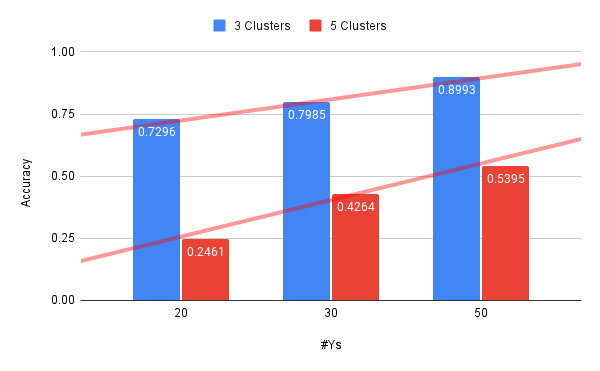
\includegraphics[width=\textwidth]{images/experiments/3_vs_5_clusters}
  \end{subfigure}
  \caption{Prediction Accuracy Bar plot for difference Ys for 3 clusters vs 5 clusters}
  \label{fig:3vs5}
\end{figure}

\begin{table}[htbp!]
  \centering
  % Title above all tables
  \caption*{\textbf{Confusion matrix of different number of Clusters with various Ys}}

  \begin{minipage}{0.45\textwidth}
    \centering
    \begin{tabular}{c|c|c|c|c}
      & \textbf{Reference} & \textbf{1} & \textbf{2} & \textbf{3} \\
      \hline
      \textbf{Prediction} & \textbf{1} & 334 & 63 & 0 \\
                          & \textbf{2} & 110 & 383 & 152 \\
                          & \textbf{3} & 1 & 39 & 268 \\
    \end{tabular}
    \caption{3 Clusters with 20 Ys}
    \label{tab:3_clu_20}
  \end{minipage}
\hfill
\begin{minipage}{0.45\textwidth}
  \centering
  \begin{tabular}{c|c|c|c|c|c|c}
    & \textbf{Reference} & \textbf{1} & \textbf{2} & \textbf{3} & \textbf{4} & \textbf{5} \\
    \hline
    \textbf{Prediction} & \textbf{1} & 0 & 0 & 0 & 0 & 0 \\
                        & \textbf{2} & 505 & 201 & 69 & 6 & 0 \\
                        & \textbf{3} & 0 & 0 & 0 & 0 & 0 \\
                        & \textbf{4} & 243 & 543 & 730 & 722 & 731 \\
                        & \textbf{5} & 0 & 0 & 0 & 0 & 0 \\
  \end{tabular}
  \caption{5 Clusters with 20 Ys}
  \label{tab:5_clu_20}
\end{minipage}

\vspace{1em} % Space between rows

  % First row of tables (2 side by side)
  \begin{minipage}{0.45\textwidth}
    \centering
    \begin{tabular}{c|c|c|c|c}
              & \textbf{Reference} & 1 & 2 & 3 \\
    \hline
    \textbf{Prediction} & 1 & 424 & 121 & 1 \\
                        & 2 & 21 & 304 & 69 \\
                        & 3 & 0 & 60 & 350 \\
    \end{tabular}
    \caption{3 Clusters with 30 Ys}
    \label{tab:3_clu_30}
  \end{minipage}
  \hfill
  \begin{minipage}{0.45\textwidth}
    \centering
    \begin{tabular}{c|c|c|c|c|c|c}
      & \textbf{Reference} & \textbf{1} & \textbf{2} & \textbf{3} & \textbf{4} & \textbf{5} \\
      \hline
      \textbf{Prediction} & \textbf{1} & 725 & 546 & 276 & 50 & 2 \\
                          & \textbf{2} & 0 & 0 & 0 & 0 & 0 \\
                          & \textbf{3} & 23 & 197 & 508 & 562 & 363 \\
                          & \textbf{4} & 0 & 0 & 0 & 0 & 0 \\
                          & \textbf{5} & 0 & 1 & 15 & 116 & 366 \\
    \end{tabular}
    \caption{5 Clusters with 30 Ys}
    \label{tab:5_clu_30}
  \end{minipage}

  \vspace{1em} % Space between rows

  % Second row of tables (2 side by side)
  \begin{minipage}{0.45\textwidth}
    \centering
    \begin{tabular}{c|c|c|c|c}
              & \textbf{Reference} & 1 & 2 & 3 \\
    \hline
    \textbf{Prediction} & 1 & 417 & 30 & 0 \\
                        & 2 & 28 & 424 & 47 \\
                        & 3 & 0 & 31 & 373 \\
    \end{tabular}
    \caption{3 Clusters with 50 Ys}
    \label{tab:3_clu_50}
  \end{minipage}
  \hfill
  \begin{minipage}{0.45\textwidth}
    \centering
    \begin{tabular}{c|c|c|c|c|c|c}
      & \textbf{Reference} & \textbf{1} & \textbf{2} & \textbf{3} & \textbf{4} & \textbf{5} \\
      \hline
      \textbf{Prediction} & \textbf{1} & 278 & 35 & 1 & 0 & 0 \\
                          & \textbf{2} & 428 & 389 & 88 & 2 & 0 \\
                          & \textbf{3} & 42 & 318 & 586 & 252 & 30 \\
                          & \textbf{4} & 0 & 2 & 121 & 423 & 354 \\
                          & \textbf{5} & 0 & 0 & 3 & 51 & 347 \\
    \end{tabular}
    \caption{5 Clusters with 50 Ys}
    \label{tab:5_clu_50}
  \end{minipage}

\end{table}

\clearpage

\subsection{Prediction with Normal Distribution Simulation}

In this set of experiments, we evaluated the clustering performance of the Ordered Stereotype Model (OSM) using different Normal distribution simulations. 
The experiments were conducted exclusively for two clusters, incorporating column effects to understand how the model performs under varying conditions. 
The EM algorithm was applied consistently across all experiments, with the number of EM cycles set to 100, the start EM cycles set to 5, and the number of starts (\textit{nstarts}) set to 5.

Figure~\ref{fig:dist_acc} presents the prediction accuracy for three distinct scenarios: "Close center," "Far center," and "Different distributions with the same cuts." 
The model's performance in all scenarios was highly effective, achieving accuracy values close to or equal to 1. Specifically, the prediction accuracy for the "Close center" scenario reached 0.99, while the accuracy for both the "Far center" and "Different distributions with the same cuts" scenarios was 1. 
These results indicate the robustness of the model under various Normal distribution configurations.

The confusion matrices for these experiments are provided in Tables~\ref{tab:nor_close}, \ref{tab:nor_far}, and \ref{tab:nor_cuts}, which provide a more detailed view of the model's classification results. 
For the "Close center" scenario (Table~\ref{tab:nor_close}), there were only 3 instances misclassified out of 300 total samples, highlighting the model's ability to distinguish between clusters even when their centers are relatively close. 
In contrast, for both the "Far center" (Table~\ref{tab:nor_far}) and "Different distributions with the same cuts" (Table~\ref{tab:nor_cuts}) scenarios, no misclassifications were observed, resulting in perfect accuracy for these experiments.

\subsubsection*{Analysis and Insights}

The high accuracy achieved across different Normal distribution configurations indicates the strength of the OSM-based clustering model in handling various data distributions. 
The slight drop in accuracy observed in the "Close center" scenario suggests that when cluster centers are very close to each other, the model faces a minor challenge in distinguishing between the clusters. 
This is a reasonable outcome, as closer cluster centers inherently introduce overlap in the data, making separation more difficult. 
Despite this, the misclassification rate remains extremely low, demonstrating that the model is still highly reliable even in more challenging scenarios.

For the "Far center" scenario, the cluster centers were further apart, which led to perfect classification accuracy. 
This indicates that the separation between clusters plays a crucial role in determining the model's performance, with greater distances leading to more distinct cluster assignments. 
Similarly, the "Different distributions with the same cuts" scenario also resulted in perfect accuracy, suggesting that the choice of cuts does not significantly impact performance when the underlying cluster centers are adequately separated.

\subsubsection*{Summary}

Overall, the results indicate that the OSM-based clustering model can effectively distinguish between clusters even under challenging Normal distribution configurations. 
The near-perfect accuracy highlights the model's capacity to handle different cluster scenarios, demonstrating its reliability for tasks involving normally distributed data. 
The slight misclassification observed in the "Close center" scenario suggests that the closeness of the cluster centers may introduce a minor degree of ambiguity, but it remains negligible in the context of overall performance. 
These insights provide confidence in the consistency of the OSM approach for clustering ordinal data, particularly when adequate cluster separation is achievable.

\begin{figure}[htbp!]
  \centering
  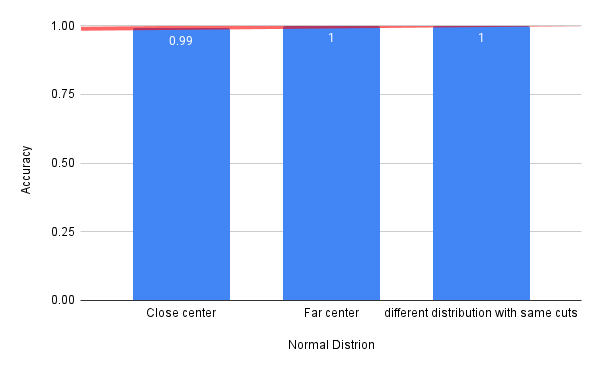
\includegraphics[width=0.8\textwidth]{images/experiments/norm_dist.png}
  \caption{Prediction Accuracy for Normal with different parameter and cuts}
  \label{fig:dist_acc}
\end{figure}


\begin{table}[htbp!]
  \centering

  % Title above all tables
  \caption*{\textbf{Confusion matrix of Normal Distributions}}

  \begin{minipage}{0.45\textwidth}
    \centering
    \begin{tabular}{c|c|c|c}
              & \textbf{Reference} & 1 & 2 \\
    \hline
    \textbf{Prediction} & 1 & 144 & 0 \\
                        & 2 & 3 & 153 \\
    \end{tabular}
    \caption{Close center}
    \label{tab:nor_close}
  \end{minipage}
  \hfill
  \begin{minipage}{0.45\textwidth}
    \centering
    \begin{tabular}{c|c|c|c}
              & \textbf{Reference} & 1 & 2 \\
    \hline
    \textbf{Prediction} & 1 & 147 & 0 \\
                        & 2 & 0 & 153 \\
    \end{tabular}
    \caption{Far center}
    \label{tab:nor_far}
  \end{minipage}

  \vspace{1em} % Space between rows

  \begin{minipage}{0.45\textwidth}
    \centering
    \begin{tabular}{c|c|c|c}
              & \textbf{Reference} & 1 & 2 \\
    \hline
    \textbf{Prediction} & 1 & 147 & 0 \\
                        & 2 & 0 & 153 \\
    \end{tabular}
    \caption{medium center}
    \label{tab:nor_cuts}
  \end{minipage}
\end{table}

\begin{figure}[htbp!]
  \centering
  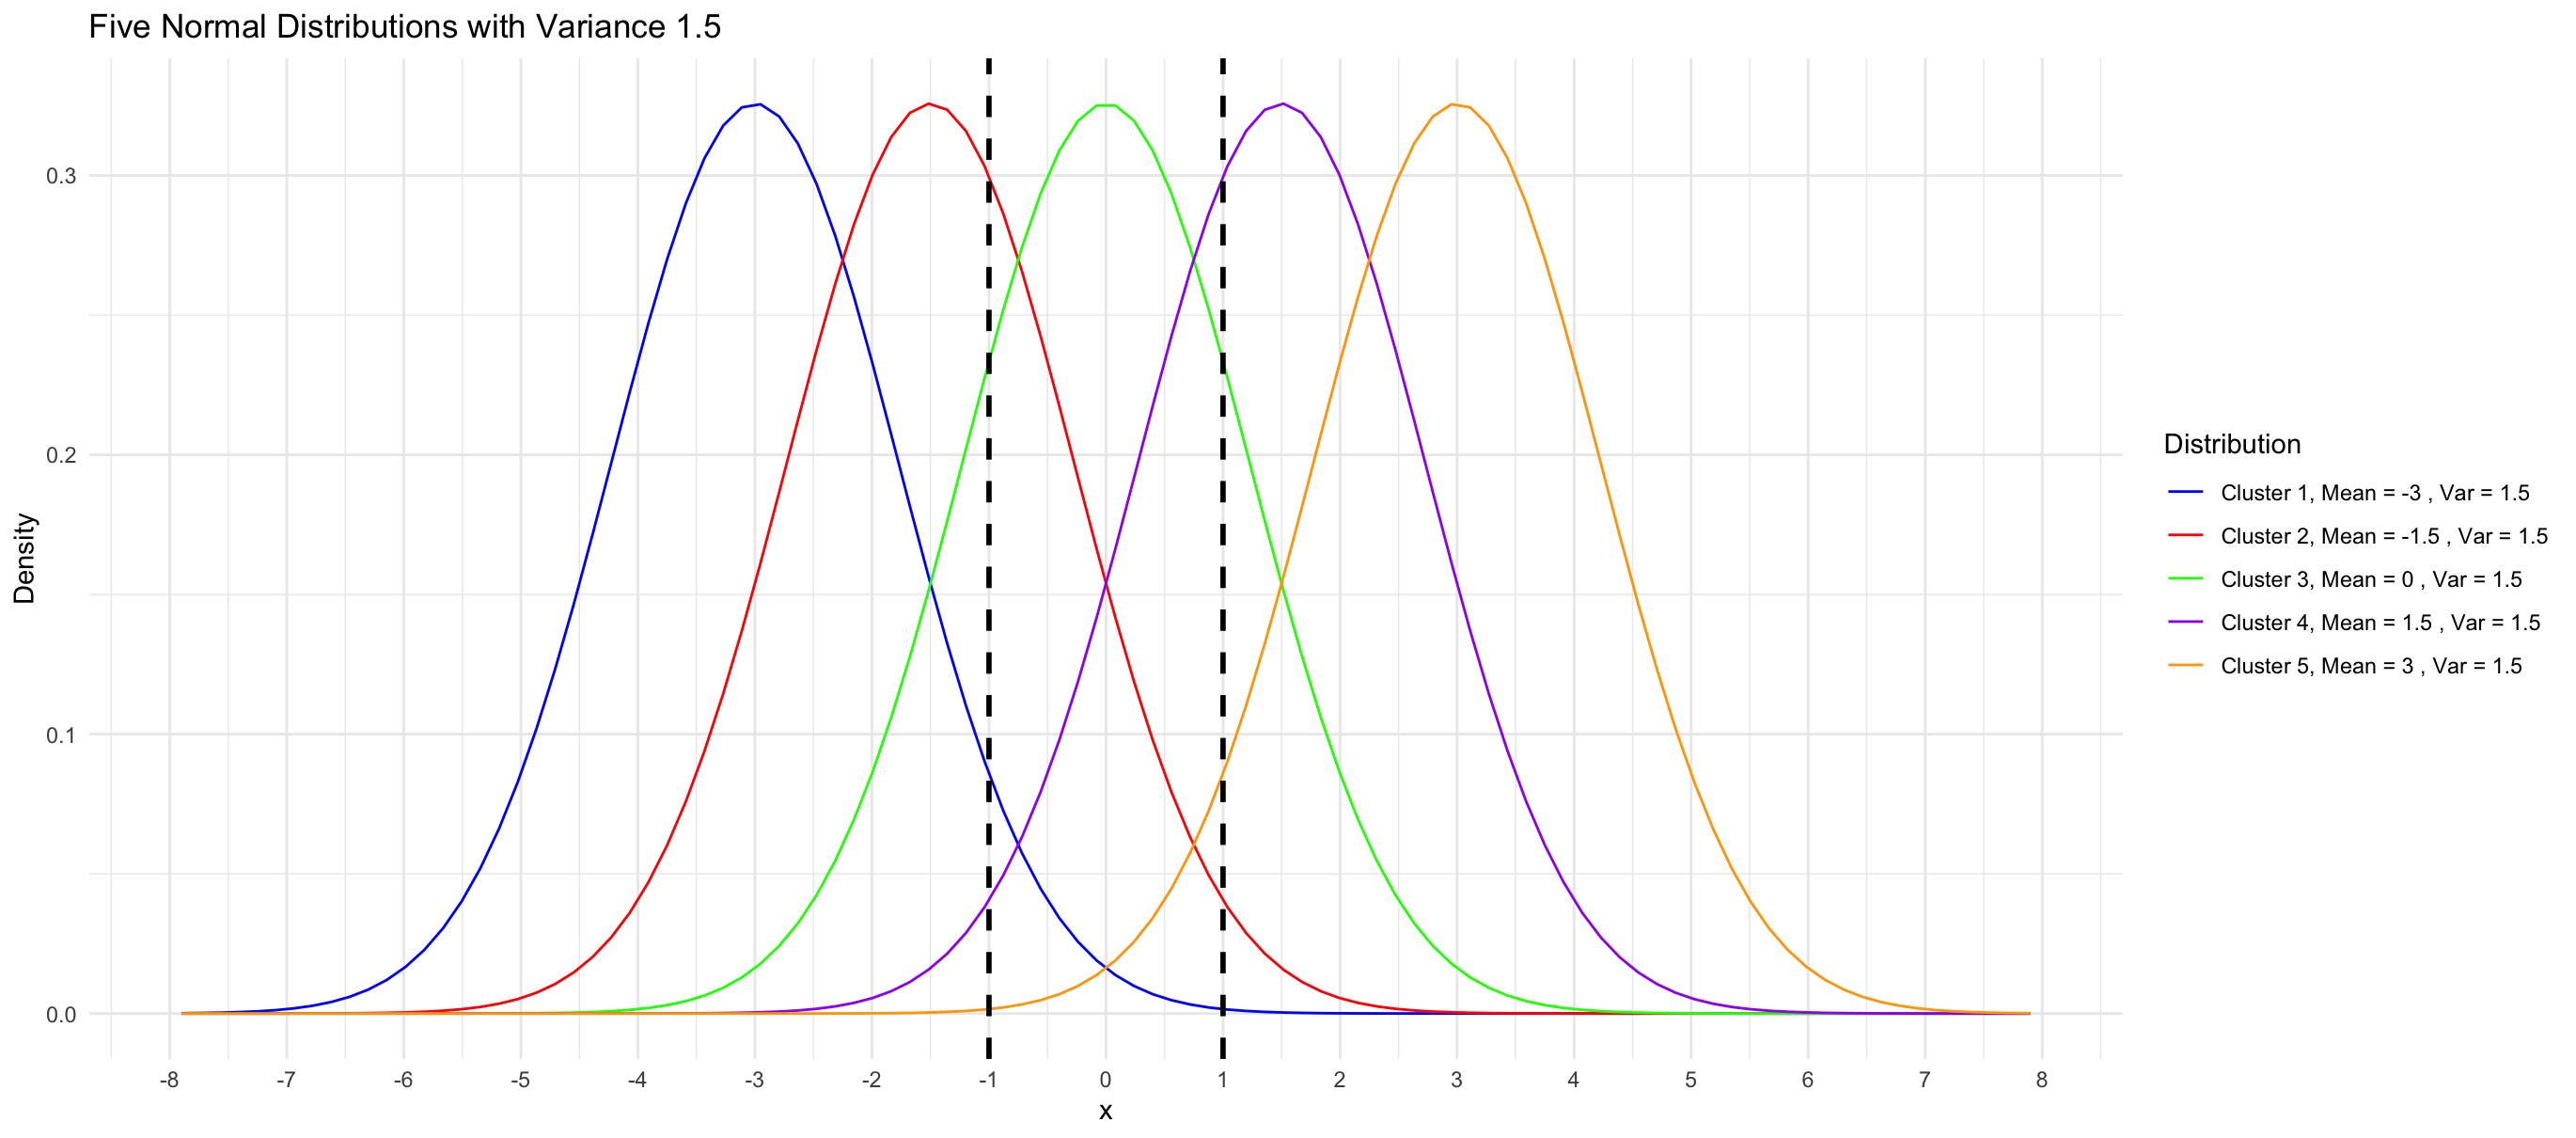
\includegraphics[width=0.8\textwidth]{images/dist_simu/dist_5_clusters.png}
  \caption{Normal Distribution Simulations for 5 clusters and 3 categories with same cuts at -1 and 1.
   (The sample value if less then cut 1 is category 1, between cut 1 and cut 2 is category 2, and larger than cut 2 is category 3.)
  }
  \label{fig:dist_5_clus}
\end{figure}

% end of Normal Dist experiment

\clearpage

\subsection{Compare prediction results between OSM simulation with Noraml simulation}

In this section, we based on 5 clusters prediciton result to compare the prediciton result performance between OSM simulation with Normal simulation.
both of these two experiments are based on 2500 observations for each cluster, which is 7500 simulation observations in total. 

The Normal Distribution simulation with 100 Ys and following distributions metioned in Figure \ref{fig:dist_5_clus}.

The OSM simulation with 100 Ys, 3 categories and $\beta$ generated from uniform Distribution. The rest parameters are following

The difference in accuracy between the two tables (0.9419 vs. 1.0) highlights that the model performs more consistently with the Normal Distribution simulation, achieving flawless accuracy. 
In contrast, the OSM simulation shows slight variability, indicating that the model may encounter some challenges when the data distribution is more complex or varied, as represented in the OSM setup.

\[
\begin{aligned}
\alpha &= \mathbf{c}(-2, -1, 0, 1, 2), \\
\mu &= \mathbf{c}(0, 0, 0), \\
\phi &= \mathbf{c}(0, 0.5, 1), \\
\pi &= \mathbf{c}(0.2, 0.2, 0.2, 0.2, 0.2).
\end{aligned}
\]

\begin{table}[htbp!]
  \centering

  % Title above all tables
  \caption*{\textbf{Confusion Matrix of Different Number of Clusters with 100 Ys}}

  \begin{minipage}{\textwidth}
    \centering
    \begin{tabular}{c|c|c|c|c|c|c}
      & \textbf{Reference} & \textbf{1} & \textbf{2} & \textbf{3} & \textbf{4} & \textbf{5} \\
      \hline
      \textbf{Prediction} & \textbf{1} & 713 & 36 & 0 & 0 & 0 \\
                          & \textbf{2} & 35 & 680 & 18 & 0 & 0 \\
                          & \textbf{3} & 0 & 28 & 762 & 20 & 0 \\
                          & \textbf{4} & 0 & 0 & 19 & 682 & 36 \\
                          & \textbf{5} & 0 & 0 & 0 & 26 & 695 \\
    \end{tabular}
    \caption{5 Clusters Prediction with 100 Ys OSM simulation}
    \label{tab:5_clu_100_ys}
  \end{minipage}
  \vspace{1cm} % Add some space between the two tables
  
  \begin{minipage}{\textwidth}
    \centering
    \begin{tabular}{c|c|c|c|c|c|c}
      & \textbf{Reference} & \textbf{1} & \textbf{2} & \textbf{3} & \textbf{4} & \textbf{5} \\
      \hline
      \textbf{Prediction} & \textbf{1} & 749 & 0 & 0 & 0 & 0 \\
                          & \textbf{2} & 0 & 733 & 0 & 0 & 0 \\
                          & \textbf{3} & 0 & 0 & 810 & 0 & 0 \\
                          & \textbf{4} & 0 & 0 & 0 & 737 & 0 \\
                          & \textbf{5} & 0 & 0 & 0 & 0 & 721 \\
    \end{tabular}
    \caption{5 Clusters Prediction with 100 Ys Normal Distribution simulation}
    \label{tab:5_clu_norm_dist}
  \end{minipage}

\end{table}

\clearpage

\section{Replication of Experiment}

To verify the consistency and robustness of our findings, we conducted a replication of the original experiment under different conditions by employing multiple runs with randomly generated seeds. The replication process involved repeating the experiment multiple times, each with a distinct random seed, to assess the variability in the obtained results.

For the replication, we used a two-cluster prediction experiment to evaluate consistency. The parameters in this replication experiment were identical to those specified in Section 9.1, ensuring comparability with prior analyses. We simulated 1,000 observations for each cluster and repeated the replication process 10 times to assess the stability and accuracy of the model's performance across these replicated trials.
Specifically, we focused on evaluating the stability of the model's performance by examining the accuracy metrics across these replicated runs. For each run, the model was trained and tested using identical parameters and data configurations, except for the random initialization determined by the seed value. We computed the accuracy for each replicate and subsequently calculated the standard deviation (std) of the accuracy scores.

The standard deviation of the accuracy across replicates serves as an indicator of the reliability of the experiment. A low standard deviation suggests that the model consistently achieves similar performance regardless of the random initialization, demonstrating the robustness of the experiment. Conversely, a higher standard deviation may indicate sensitivity to the initial conditions, suggesting a need for further investigation into factors contributing to this variability.

Our results showed that the standard deviation of accuracy across the replicated experiments was 
0.0083
, indicates that the model’s performance is highly consistent across different initializations.

The low standard deviation demonstrates that the model’s accuracy remains relatively stable, suggesting
that the training process and resulting predictions are not overly sensitive to the random initialization. 
This consistency highlights the robustness of the model and provides confidence that the
reported accuracy is representative and not merely a result of favorable initial conditions.
Overall, the replication analysis supports the reliability of our experimental results, indicating that our
model produces stable predictions irrespective of the variability introduced by different random seeds.


\section{Conclusion and Future Directions}

In this paper, we extended the clustering methodology for ordinal data using the Ordered Stereotype Model (OSM) within the framework of Finite Mixture Models (FMM). We focused on enabling the prediction of cluster membership for new, unlabeled data. This extension is crucial for applying ordinal data analysis in dynamic environments where new data is continuously generated, requiring efficient and accurate classification. Our approach involved constructing a prediction function that, after model parameter estimation, allows for direct cluster assignment of new observations, supported by both OSM simulations and Normal distribution-based simulations.

We conducted experiments that systematically varied parameters such as the number of response variables (\( Y \)) and the number of clusters (\( G \)), as well as different configurations of the OSM model parameters (\(\alpha\), \(\mu\), \(\phi\), \(\beta\), and \(\pi\)). Our results demonstrated that the model's clustering performance improves with an increased number of response variables and that prediction accuracy decreases significantly as the number of clusters increases, emphasizing the importance of balancing model complexity with available information. The experiments with Normal distribution-based simulations further validated the robustness of our approach, with near-perfect accuracy across different cluster scenarios.

We also addressed the issue of label switching, a common challenge in clustering algorithms that employ the Expectation-Maximization (EM) approach. By implementing a reordering step to consistently align cluster labels based on the estimated probabilities of the latent variable \(\alpha\), we were able to mitigate the label switching problem, ensuring reliable evaluation of model predictions across multiple runs.

The replication study revealed the robustness of our model, with a low standard deviation of prediction accuracy across experiments with different random seeds, reinforcing the consistency of the model's performance. This highlights the stability of our approach and its suitability for real-world applications where reliable clustering predictions are essential.

\subsection{Future Directions}

While the results presented in this paper show promising advancements in cluster prediction for ordinal data, several future directions could further enhance the applicability and performance of the proposed methodology:

\begin{itemize}
    \item \textbf{Integration with Machine Learning Techniques}: One potential future direction is to integrate traditional statistical models like OSM with modern machine learning techniques, such as deep learning. This hybrid approach could improve the model's ability to capture complex relationships in large, heterogeneous datasets while maintaining interpretability.

    \item \textbf{Expanding to Higher-Dimensional Data}: The current work focused on scenarios involving two to five clusters. Expanding the methodology to handle more complex, higher-dimensional data with a larger number of clusters could provide valuable insights into its scalability and efficiency. Additional research is needed to explore strategies for improving accuracy when predicting a greater number of clusters, particularly when available data is limited.

    \item \textbf{Alternative Model Structures for Ordinal Data}: Investigating alternative model structures, such as Bayesian approaches or hierarchical mixture models, may further improve clustering performance for ordinal data. These methods could provide additional flexibility in modeling the dependencies between response variables, thus enhancing predictive capabilities.

    \item \textbf{Real-World Data Validation}: Although our simulations demonstrated the robustness and effectiveness of the proposed model, future research should involve validating the model on real-world ordinal datasets from various domains, such as social sciences, healthcare, or market research. This step is critical to assess the practical utility of the model and ensure its generalizability beyond the controlled environment of simulated data.

    \item \textbf{Exploring the Impact of Covariates}: While this study considered the effect of covariates in the clustering process, future work could explore the impact of additional covariates and more complex interactions between covariates and clusters. Understanding these effects could provide deeper insights into how different factors contribute to the clustering structure, thereby improving the model's interpretability and application.

    \item \textbf{Enhanced Handling of Label Switching}: Although our deterministic relabeling strategy effectively mitigated label switching, further work is needed to develop more sophisticated techniques that can handle label switching in a wider variety of clustering contexts. This is especially important for large-scale clustering applications involving many clusters.

\end{itemize}

In conclusion, this work contributes to the existing body of literature on ordinal data analysis by extending the FMM framework to incorporate predictive clustering capabilities, supported by rigorous experimentation and analysis. The proposed methodology provides a solid foundation for future studies and opens up new avenues for effectively utilizing clustering in dynamic environments with ordinal data. We are confident that the insights gained from this research will serve as a stepping stone for further developments in the area of ordinal data clustering and prediction.


\printbibliography

\end{document}
